\documentclass[herrin-thesis.tex]{subfiles}
\begin{document}

\chapter{Electron Lifetime}
\label{ch:electronlifetime}

\section{Electron Capture on Impurities}
When an electromagnetic process deposits energy in a noble liquid detector, it ionizes the atoms, producing electrons and ions. Some of the electrons will recombine with the ions, which produces scintillation light. However, if the detector has an applied electric field, then the remaining electrons and ions will drift in opposite directions along the field lines. In a detector consisting of perfectly pure noble liquid, the electrons would all reach the anode and would be collected for an energy measurement. In a non-ideal detector, however, electronegative impurities can capture the drifting electrons and form ions. The ions are more massive and drift more slowly, and so they escape inclusion in the signal used for energy measurement.

Electronegative impurities may capture electrons in three ways\cite{Aprile:2006fk}. Denoting the impurities, which may be atoms or molecules, as \(AB\), these are:
\begin{enumerate}
\item Radiative attachment
\begin{equation}
e^{-} + AB \rightarrow AB^{-} + h \nu
\end{equation}
which has a much smaller cross section than the other processes below.
\item Dissociative attachment
\begin{equation}
\begin{split}
e^{-} + AB \rightarrow e^{-} + AB^{*} \rightarrow A^{+} + B^{-} + e^{-} \\
e^{-} + AB \rightarrow AB^{-} \rightarrow A^{+} + B^{-}
\end{split}
\end{equation}
which requires the electron's energy to be much higher than typically found for an electron drifting in a liquid or dense gas.
\item Three-body attachment through the two-stage Bloch-Bradbury reaction
\begin{equation}
\begin{split}
e^{-} + AB \leftrightarrow (AB^{-})^{*} \\
(AB^{-})^{*} + X \rightarrow AB^{-} + X
\end{split}
\label{eq:el_3bodyattachment}
\end{equation}
where X represents the atom or molecule that make up the majority of the liquid.
\end{enumerate}

The three-body reaction shown in \cref{eq:el_3bodyattachment} releases some amount of energy, given by the \emph{electron affinity} of \(AB\). The electron affinity is positive if \(AB\) is electronegative. Noble elements have a negative electron affinity, so the reaction does not take place in a pure detector.

The rate of the reaction shown in \cref{eq:el_3bodyattachment} is given by:
\begin{equation}
\frac{dn_{AB}}{dt} = -k_{3} n_{AB} n_{X} n_{e^{-}}
\label{eq:el_3bodyreactionrate}
\end{equation}
where \(k_3\) is constant for the 3-body reaction, and \(n_{AB}\), \(n_{X}\), and \(n_{e^{-}}\) are the densities of the impurity, the atoms or molecules of the liquid, and the electrons, respectively. \(k_3\) depends on the species of the impurity, the species of the liquid, and the electric field strength.

According to \cref{eq:el_3bodyreactionrate}, electrons will be captured, forming \(AB^{-}\) at a rate proportional to the density of electrons. Thus, the number of free electrons will decay exponentially over time according to:
\begin{equation}
N_{e^{-}}(t) = N_0 \exp (-t/\tau_e)
\label{eq:el_exponentialtaue}
\end{equation}
where \(N_0\) is the original number of electrons, and \(\tau_e\) is the \emph{electron lifetime}.

In general, there can be several different species of electronegative impurity. In that case, they all contribute to the electron lifetime according to:
\begin{equation}
\tau_e^{-1} = \sum_i k_i n_i = \sum_i\tau_i^{-1}
\label{eq:el_tauedefinition}
\end{equation}
where \(n_i\) is the density of an electronegative impurity and \(k_i\) is the cross section for electron capture by that impurity.

\section{Measuring Electron Lifetime}

\subsection{Method}
\Cref{eq:el_exponentialtaue} provides a simple recipe for measuring the electron lifetime: measure the exponential attenuation of a known quantity of ionization as a function of drift time. A source of monoenergetic gamma rays can provide such a signal. The ionization produced by the full absorption of a gamma ray follows a Gaussian distribution, with its width provided by the Fano factor and detector resolution. If some of the ionization is being attenuated, then the peak's mean will shift downward in energy from its true value.

A single calibration source at the cathode of the detector illuminates both TPCs, and the gamma rays interact throughout the entire drift region. After a sufficiently long calibration run, the TPC is divided into drift time bins. The size of the bins is a compromise: a larger bin in drift time will have more events, and thus the measurement of the full absorption peak energy will be better. A smaller bin will have fewer events, but will suffer less energy smearing because events will have similar drift times. In practice, 16 bins per TPC seems a good compromise.

\begin{figure}[htbp]
\centering
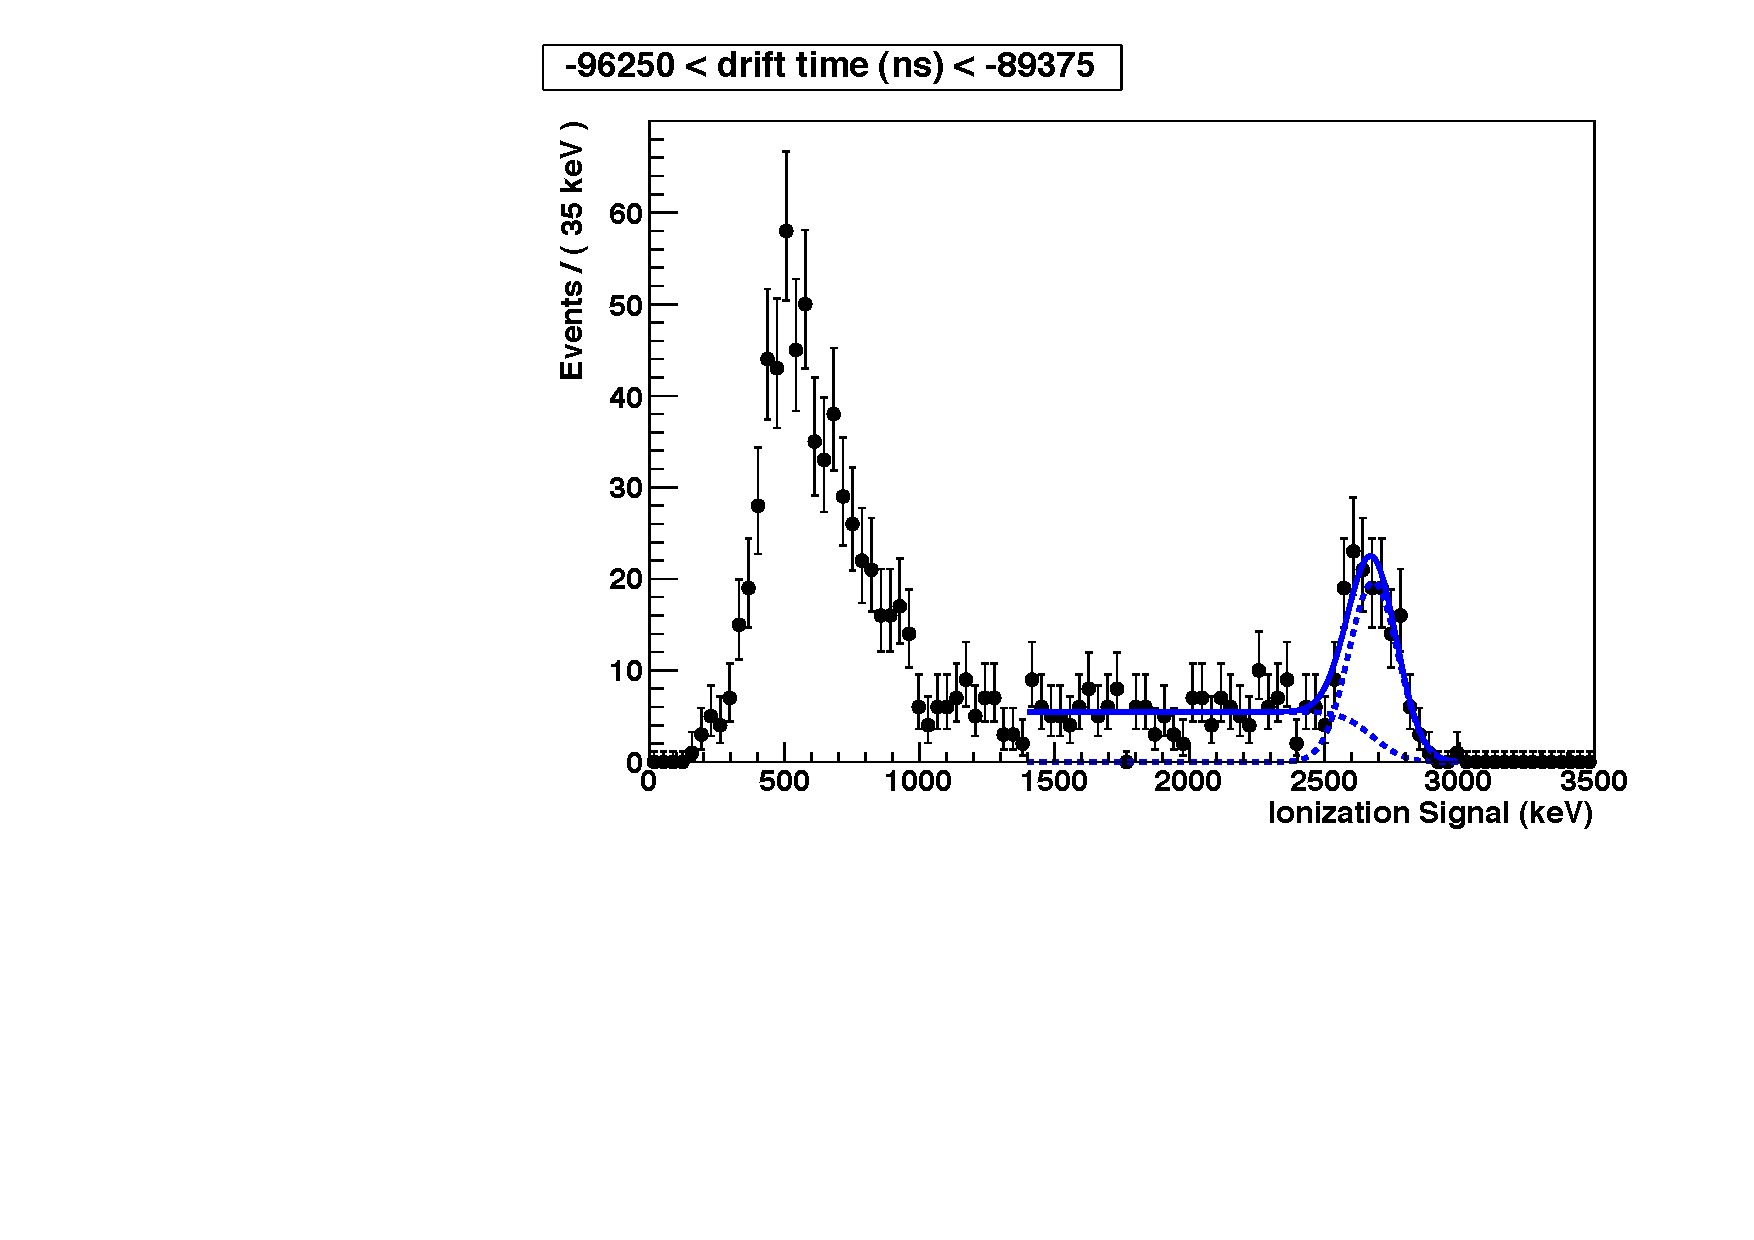
\includegraphics[width=0.6\columnwidth]{./plots/el_run4034_dt_bin_fit.pdf}
\caption[An example fit in a drift time bin]{A fit of the simple Gaussian + complementary error function model to one single drift time bin. In this example, the full absorption peak is the 2615 keV gamma line from \thorium{228}.}
\label{fig:el_dtbinfit}
\end{figure}

In addition to the full-absorption peak, which is Gaussian, the energy spectrum from a gamma ray source will contain a Compton shoulder. Some gamma rays will interact without depositing their full energy, and then scatter out of the detector. A simple model for this shoulder is a step function convolved with a Gaussian smearing representing the effects of energy resolution, producing a complementary error function. For each drift time bin, I fit this simple Gaussian + complementary error function model to the energy spectrum of that bin using an unbinned maximum likelihood fit. This fit is performed twice, first over a broad energy range to find the full-absorption peak, then in the range \((-3.0\sigma, +2.5\sigma)\) of the found peak to precisely determine the peak energy. \Cref{fig:el_dtbinfit} shows an example fit.

\begin{figure}[htbp]
\centering
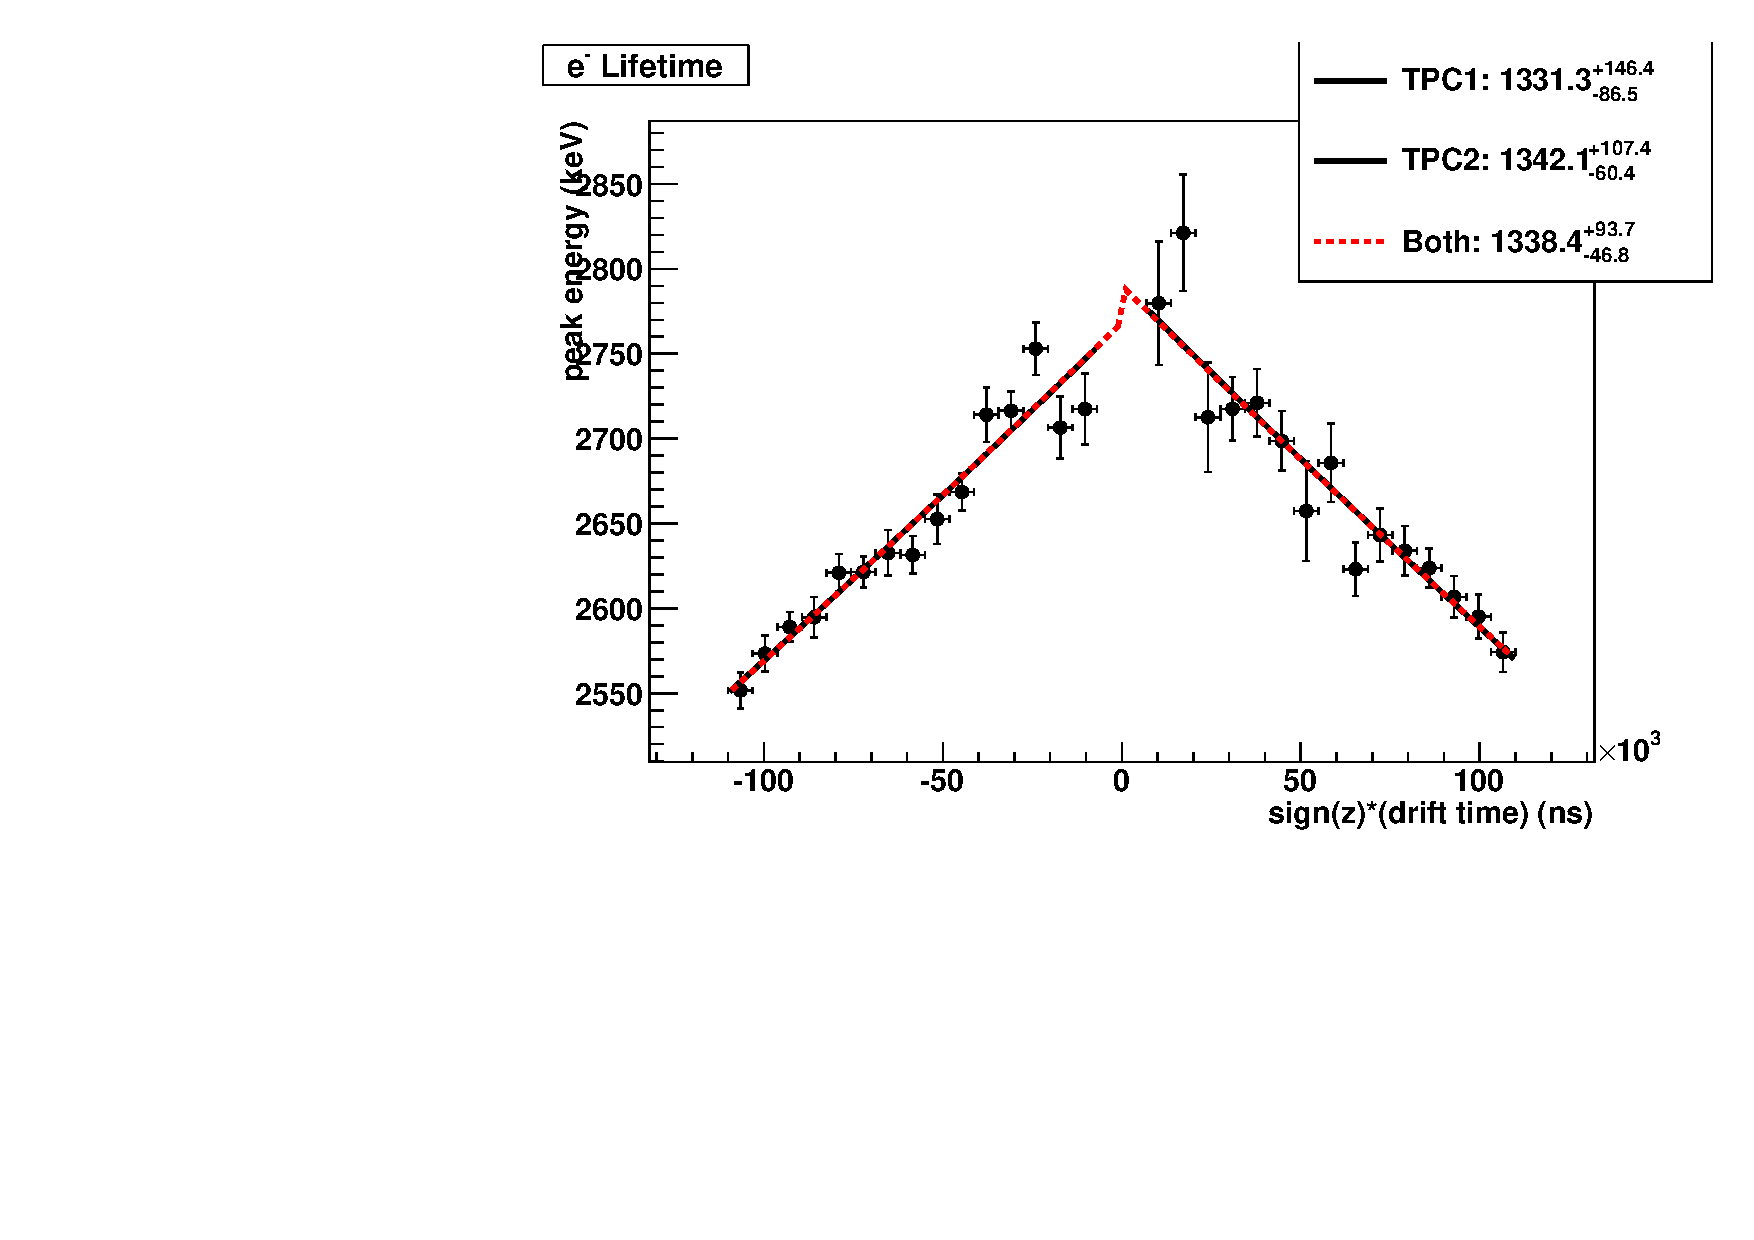
\includegraphics[width=0.6\columnwidth]{./plots/el_run4228_fit.pdf}
\caption[An example fit to exponential attenuation]{Measuring the electron lifetime by fitting a decaying exponential to the full-absorption peak energies binned by drift time. TPC 2 is assigned a negative drift time for convenience in visualization. Both fits to the individual TPCs and to both TPCs together are shown.}
\label{fig:el_elfit}
\end{figure}

Plotting the full absorption peak energy from each drift time bin as a function of drift time reveals the exponential decay described in \cref{eq:el_exponentialtaue}. Fitting an exponential to each TPC yields a measurement of the electron lifetime for each. Alternatively, a fit with a single electron lifetime to the entire detector uses information from both TPCs. In all cases, the amplitude of the exponential is allowed to float in the fit, since only the relative decay matters when measuring the electron lifetime. Presently, the separate TPC lifetimes are used when correcting for electron lifetime in EXO-200, while the single measurement is used when monitoring the detector and data quality. \Cref{fig:el_elfit} shows an example.

\begin{figure}[htb]
\centering
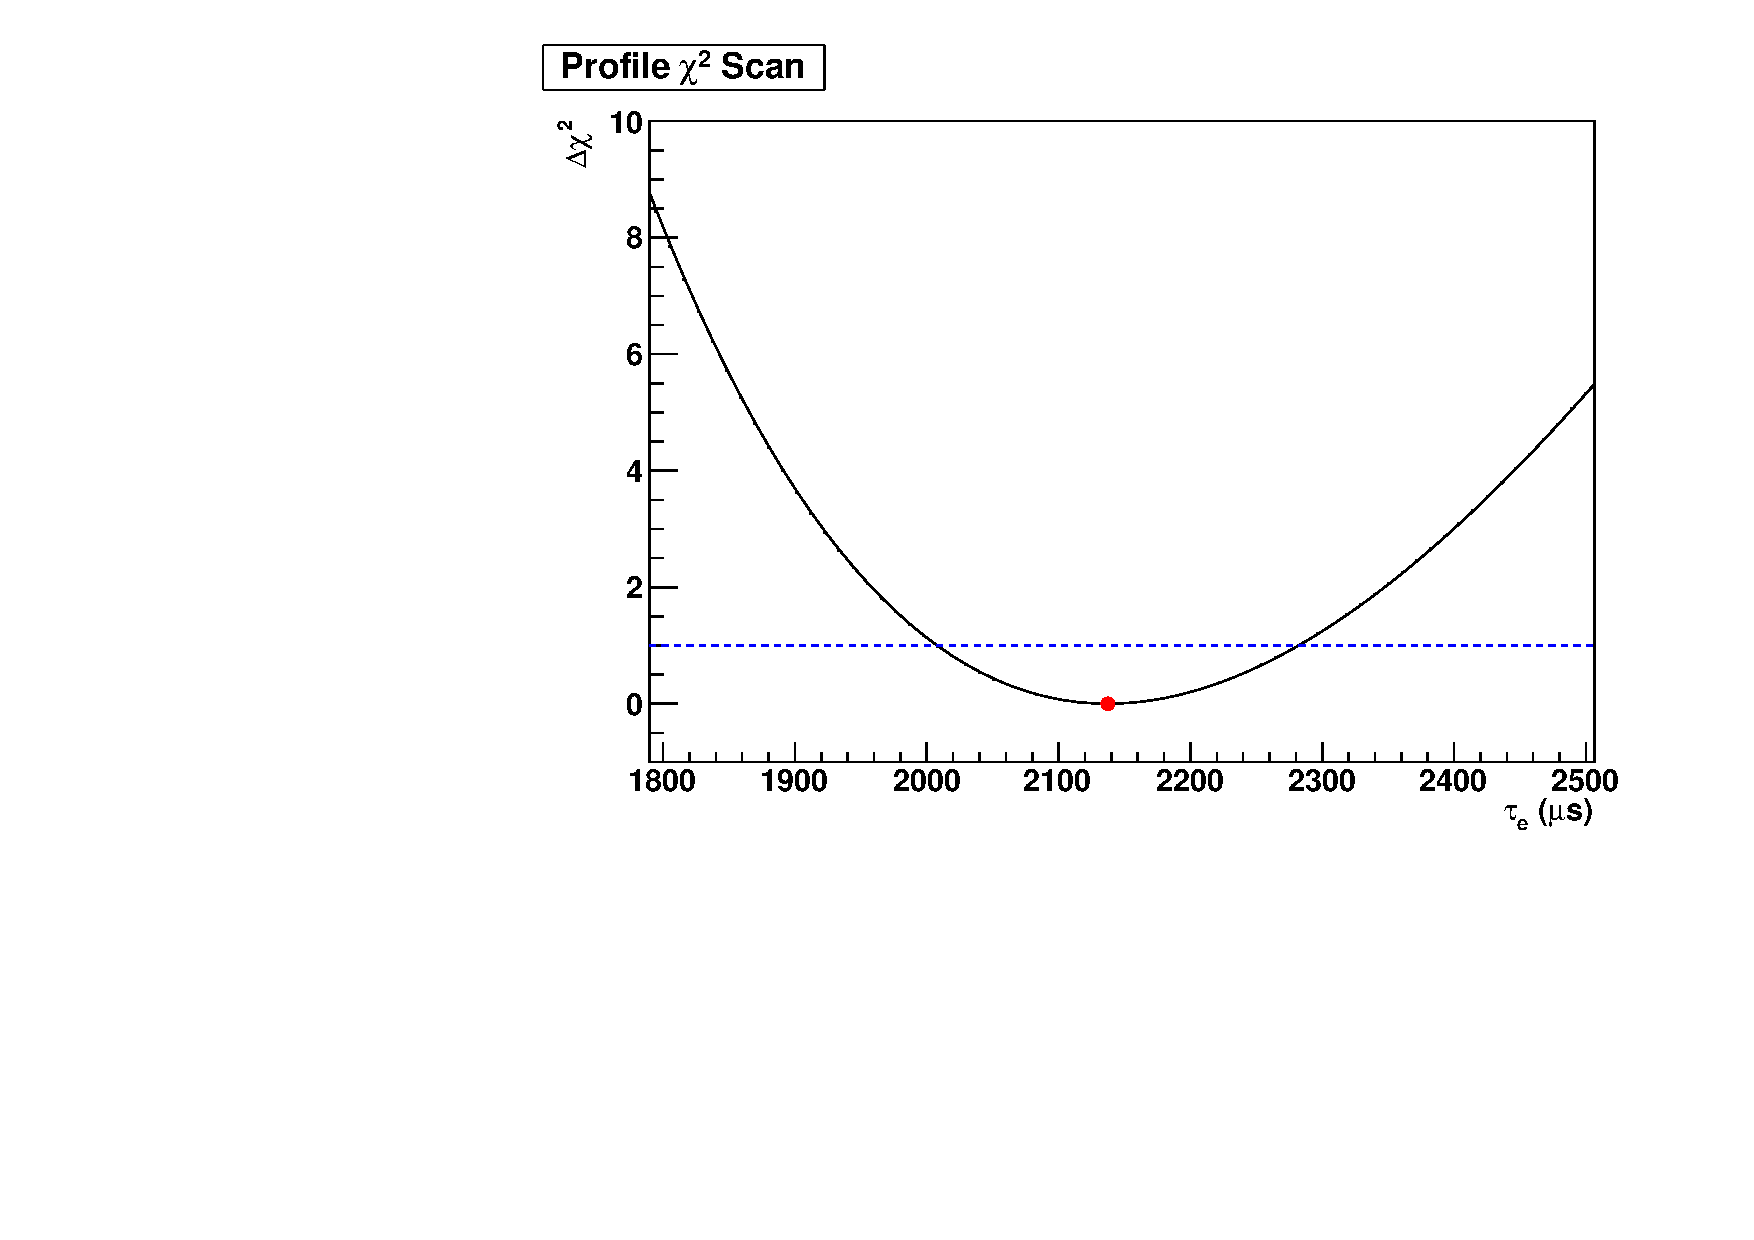
\includegraphics[width=0.6\columnwidth]{./plots/el_run4252_profile.pdf}
\caption[A profile scan around the best-fit electron lifetime]{Confidence intervals around the best fit electron lifetime come from a profile scan, shown here. As this figure shows, this is superior to simply estimating the 1\(\sigma\) errors from the second derivative at the best fit value, since the profile is asymmetric around the best fit (indicated by the red dot). The blue line indicates \(\Delta\chi^2 = 1\), corresponding to a 68\% confidence interval.}
\label{fig:el_profileel}
\end{figure}

The electron lifetime measurement comes from minimizing the \(\chi^2\) statistic. Confidence intervals for the measurement come from doing a profile scan. Short electron lifetimes are easily distinguished, while longer electron lifetimes are not, and so the intervals will be asymmetric about the minimum. For a profile scan the electron lifetime is set to some fixed value away from the best fit value, and the amplitude is allowed to vary to minimize \(\chi^2\). All electron lifetime values for which this reminimized \(\chi^2\) is less than 1 above the minimum value define the 1\(\sigma\) (68\%) confidence band. \Cref{fig:el_profileel} shows an example.

\subsection{Comparison to Simulation}

\begin{figure}[htb]
\begin{subfigure}[b]{0.5\linewidth}
\centering
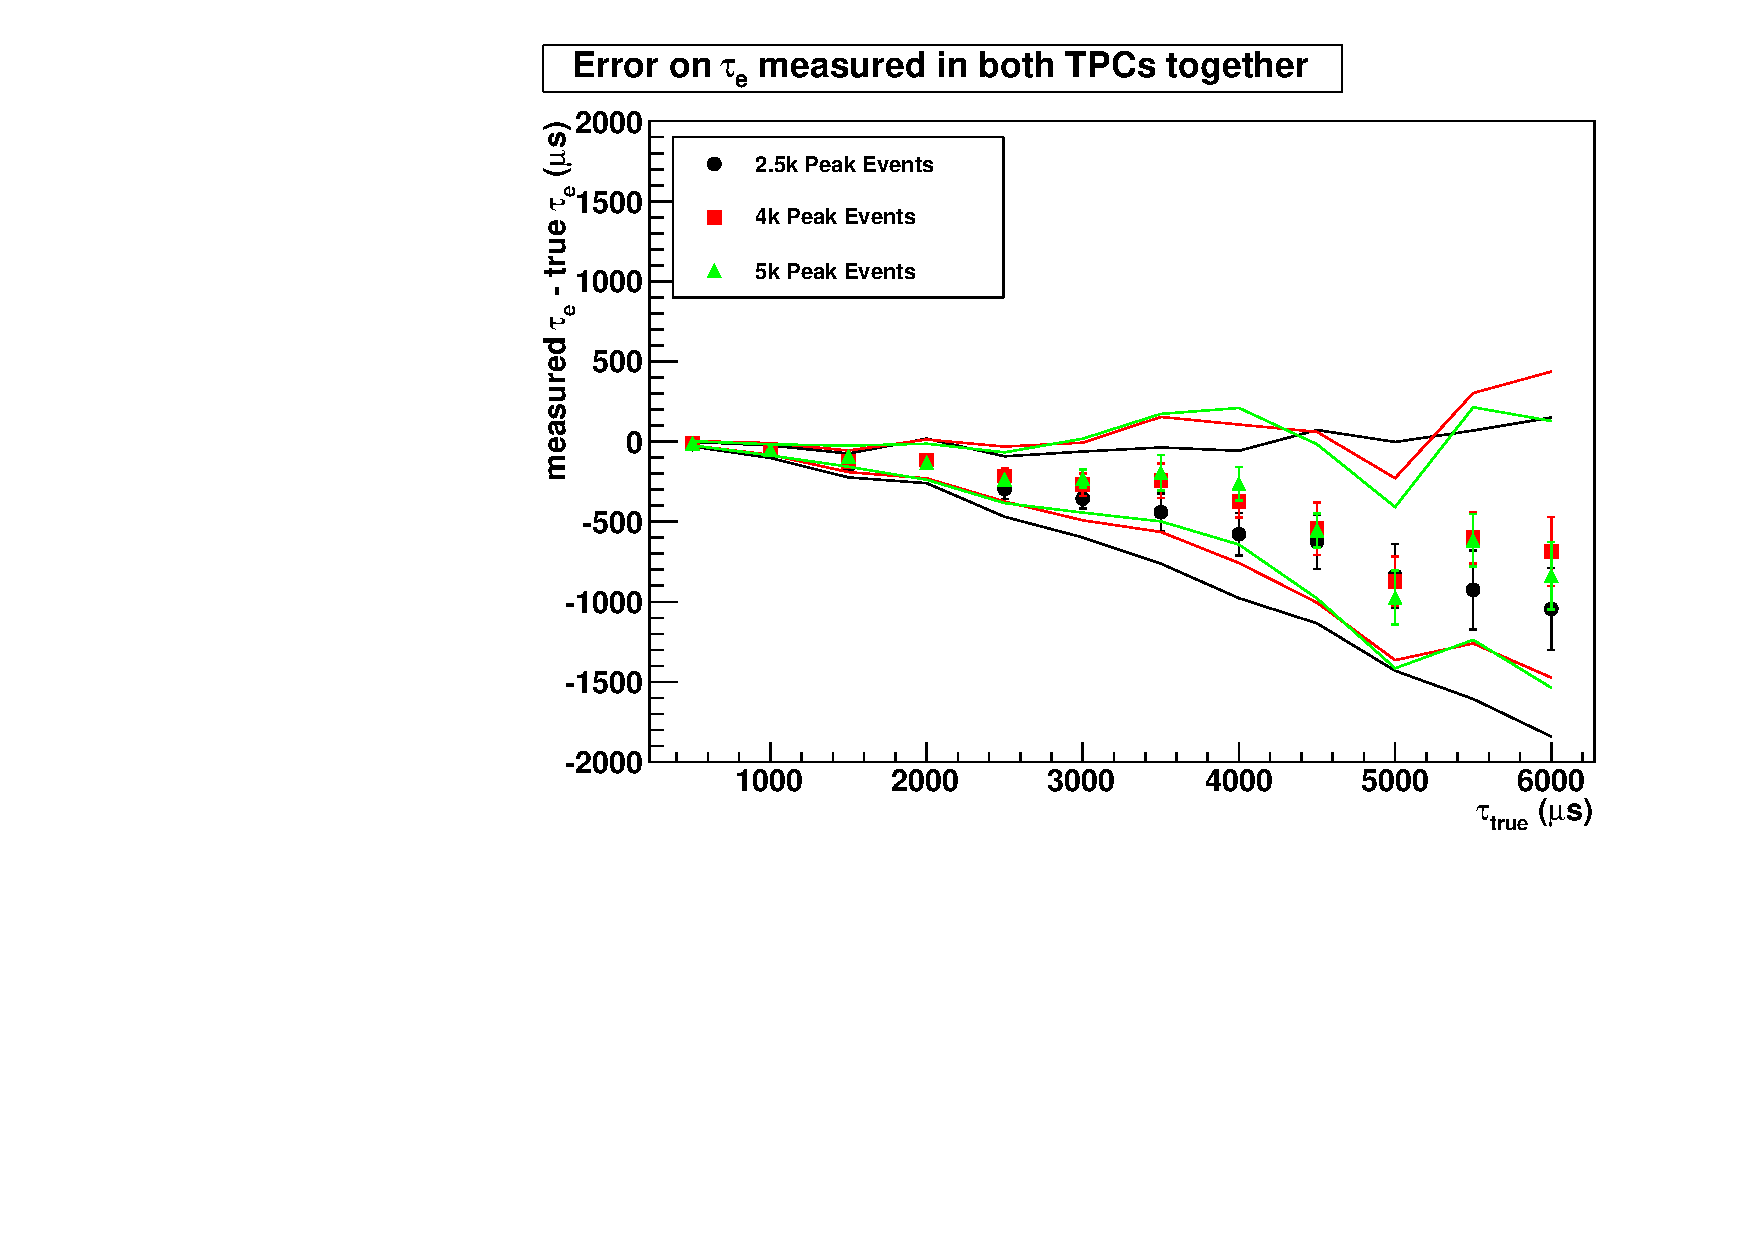
\includegraphics[width=1.0\columnwidth]{./plots/el_sim_error_both.pdf}
\end{subfigure}%
\begin{subfigure}[b]{0.5\linewidth}
\centering
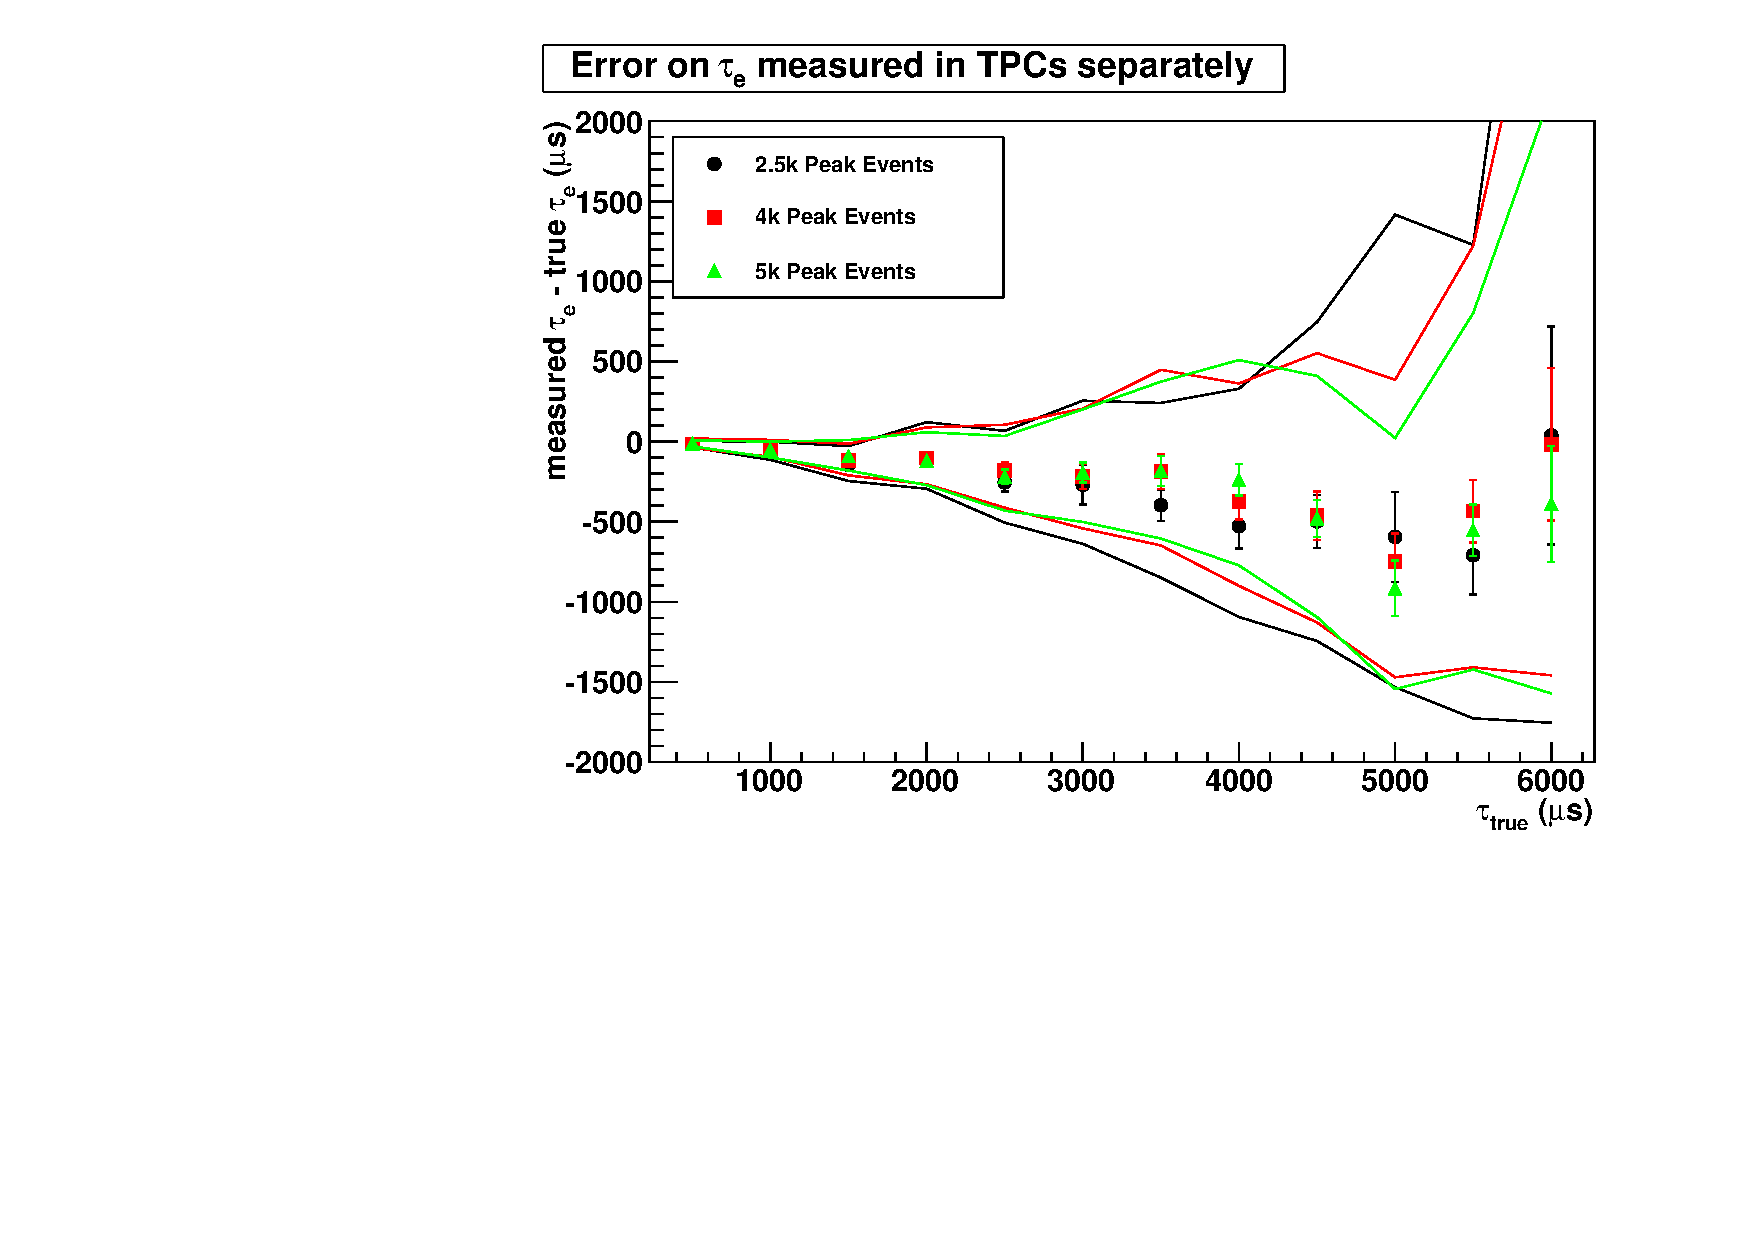
\includegraphics[width=1.0\columnwidth]{./plots/el_sim_error_indiv.pdf}
\end{subfigure}
\caption[Error on reconstructed electron lifetime from simulation]{The absolute error on the electron lifetime measurement for the electron lifetime measured in both TPCs simultaneously (left) and individually (right). The points show the mean error of 20 simulations, and the lines show the mean error on the edges of the 68\% confidence bands for those simulations. The measurement method consistently underestimates the purity, and the error grows as the electron lifetime gets large. Typical calibration runs include 2.5k events in the full absorption peak (black), but using more events would improve the error.}
\label{fig:el_sim_err}
\end{figure}

\Cref{fig:el_sim_err} shows a comparison between a known simulated electron lifetime and the measurement of that lifetime using the method described above. The error is small for electron lifetimes below \SI{1}{\ms}. For large electron lifetimes, however, the method consistently underestimates the electron lifetime, with the effect getting worse as the electron lifetime improves. 

This effect seems to be due to a some \(z\)-dependence introduced in processing the data. In simulations of a \thorium{228} source at the cathode with infinite electron lifetime, the method reports electron lifetimes of \SI{3.0\pm0.9d4}{\micro\second} measured in both TPCs simultaneously, and \SI{4.3\pm0.9d4}{\micro\second} measured in a single TPC, for runs with 2.5k events in the full absorption peak. It reports electron lifetimes of \SI{5.0\pm0.7d4}{\micro\second} measured in both TPCs simultaneously and \SI{4.9\pm0.8d4}{\micro\second} measured in a single TPC, for runs with 5k events in the full absorption peak.

The error due to this effect is small, however. A measured electron lifetime of \SI{3000}{\micro\second} corresponds to a true electron lifetime of roughly \((1/3000-1/40000)^{-1} =\) \SI{3250}{\micro\second}. This will only move the corrected ionization signal 0.3\% higher than its true value, if the ionization drifts over the full \SI{120}{\micro\second} drift time. The effect on the energy resolution in the ionization channel will be half of this this, and even smaller in the rotated spectrum. It is not understood what in the processing chain causes the effect, or if it is also present in real data. Therefore, this effect is accepted as a slight worsening in energy resolution, rather than corrected for.

\subsection{Practical Considerations}

\begin{figure}[htb]
\begin{subfigure}[b]{0.5\linewidth}
\centering
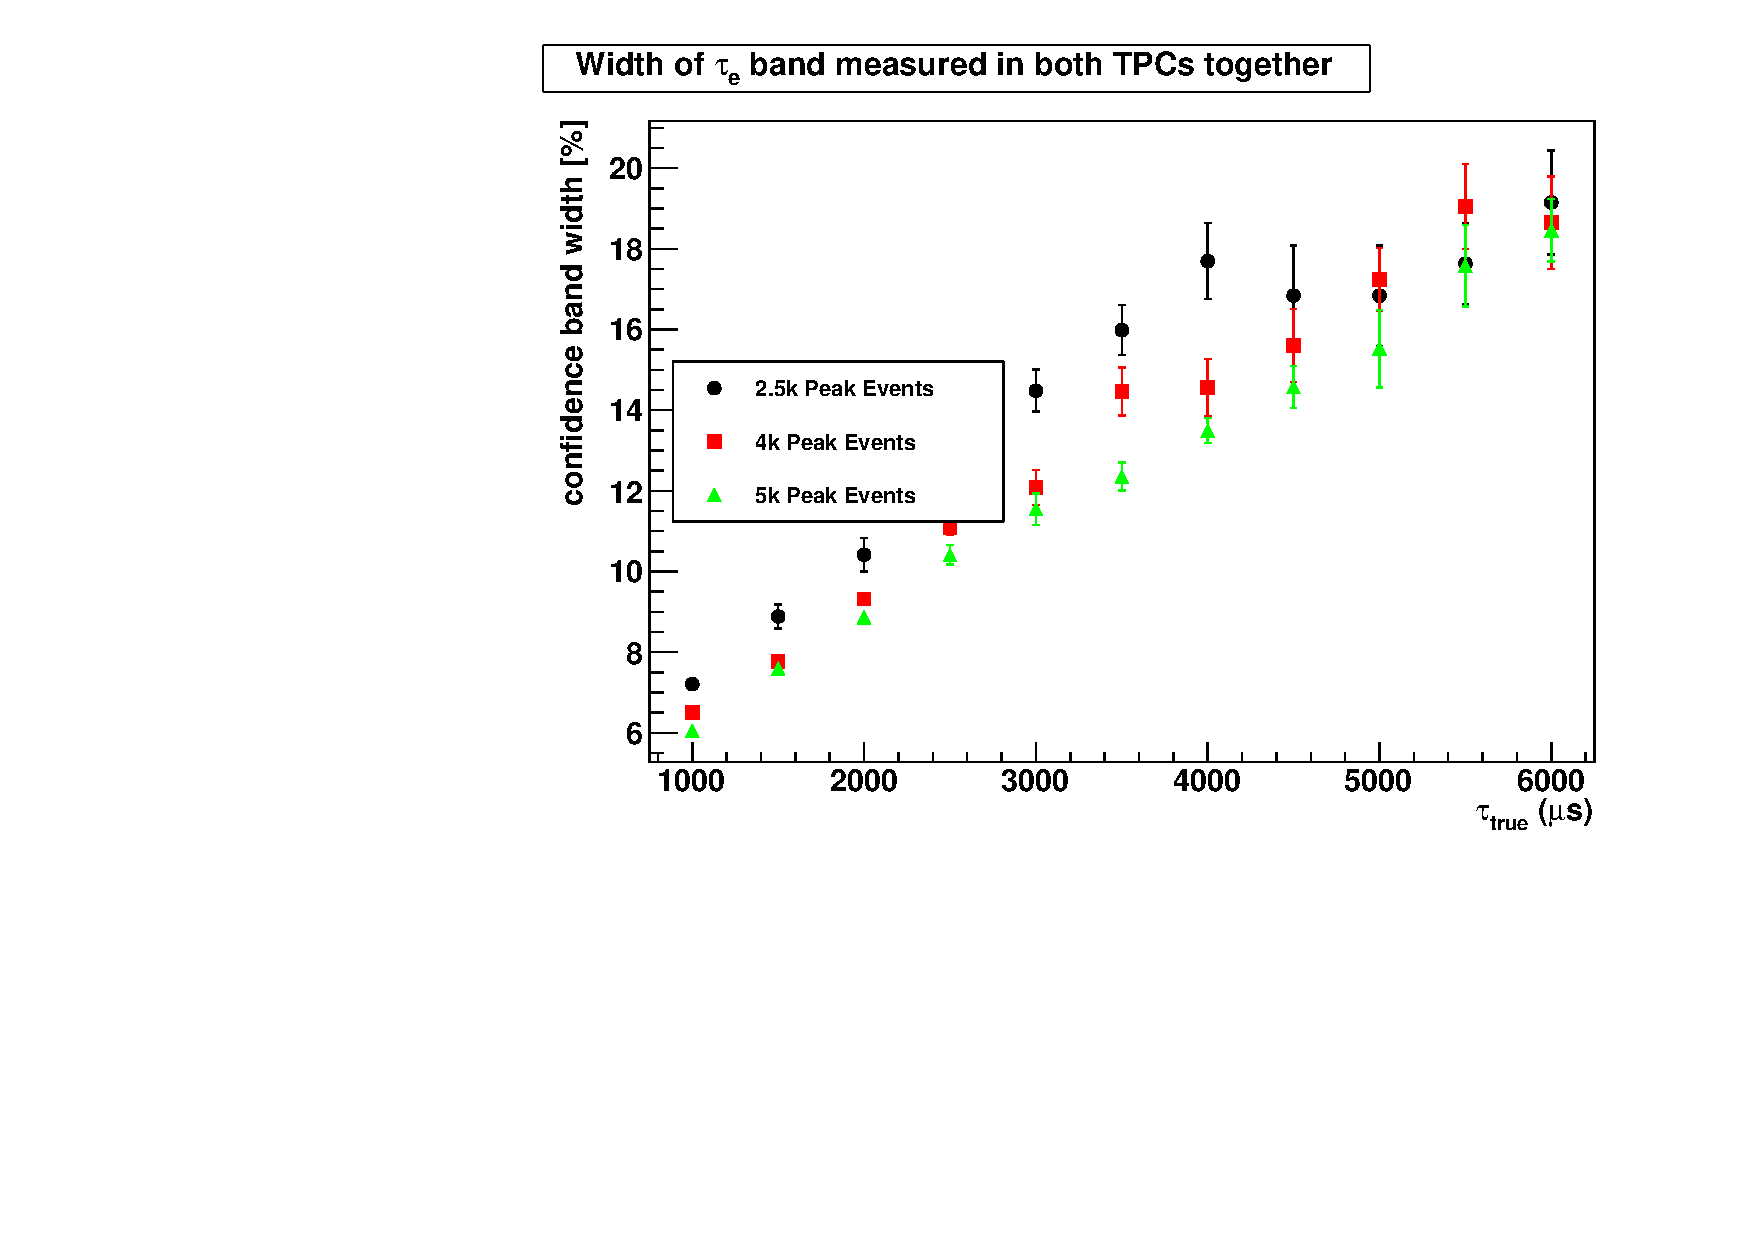
\includegraphics[width=1.0\columnwidth]{./plots/el_sim_width_both.pdf}
\end{subfigure}%
\begin{subfigure}[b]{0.5\linewidth}
\centering
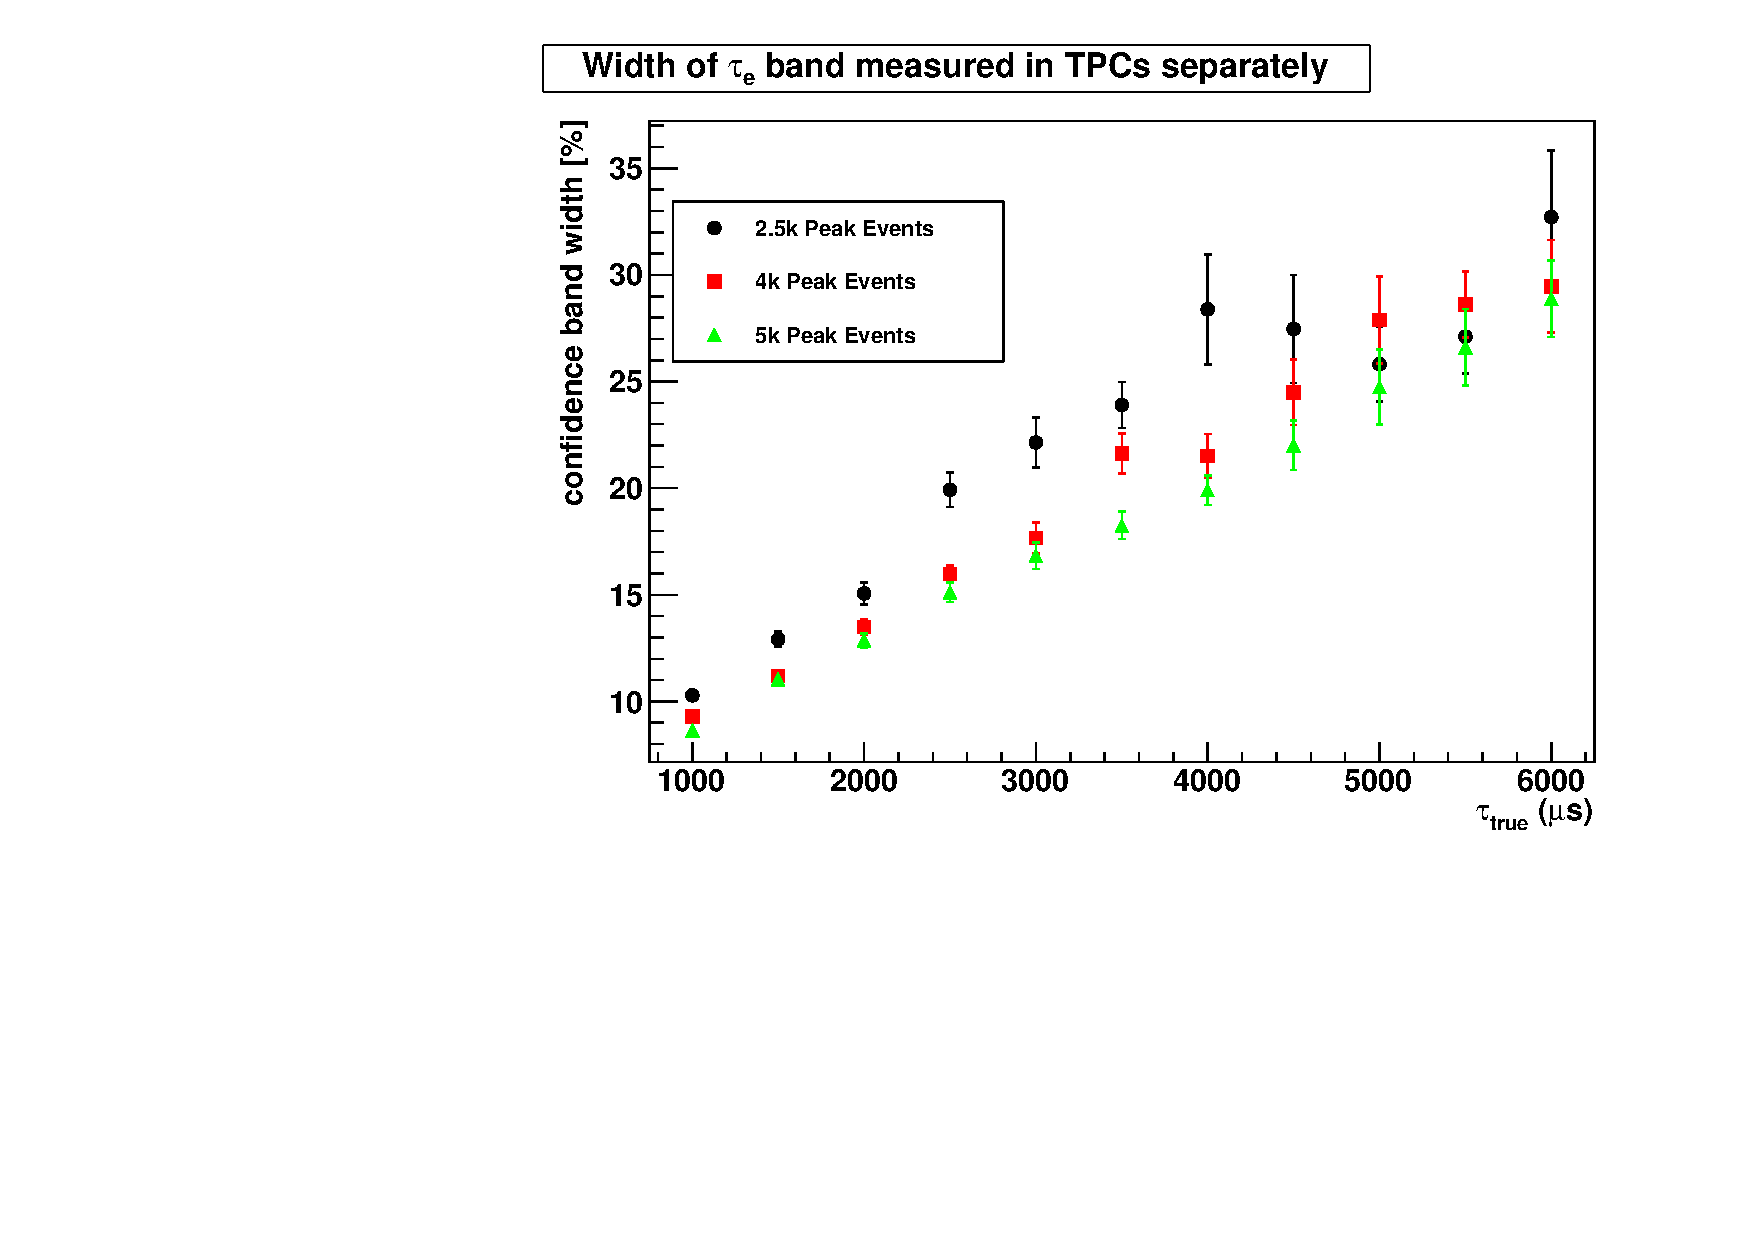
\includegraphics[width=1.0\columnwidth]{./plots/el_sim_width_indiv.pdf}
\end{subfigure}
\caption[Confidence band widths for electron lifetime measurements]{The width of the 68\% confidence band for the electron lifetime measured in both TPCs simultaneously (left) and individually (right). Typical calibration runs include 2.5k events in the full absorption peak (black dots), but using more events would improve the error. Using longer calibrations would improve the uncertainty. However, for long electron lifetimes, it becomes difficult to detect the attenuation and measure it, giving a large uncertainty.}
\label{fig:el_sim_width}
\end{figure}

As the electron lifetime grows large, it becomes increasingly difficult to measure. For a \SI{4000}{\micro\second} electron lifetime, ionization drifting the full distance will only be attenuated about 3\%. This is comparable to the 3.4\%\todo{May need to be updated} energy resolution in the ionization channel at the 2615 keV full absorption peak from \thorium{228}. This effect is shown in \cref{fig:el_sim_width}. The width of the confidence band for the measurement grows to near 20\% of the measured value for large electron lifetimes. Taking more calibration data only partially mitigates this effect, also shown in \cref{fig:el_sim_width}. For low electron lifetimes, a simulated calibration run with twice as many events in the full absorption peak (and requiring twice as much time to run) shrinks the confidence band by roughly \(\sqrt{2}\). For large electron lifetimes, more events don't shrink the band, suggesting systematic errors such as the relatively short drift time dominate.

\section{Effects of Electron Lifetime on the Energy Resolution}

The error on \(E_{rotated}\) due to an uncertainty \(\Delta\tau\) in the electron lifetime is:
\begin{equation}
\frac{\Delta E_{rotated}}{E_{rotated}} = \cos(\theta) \frac{t_d}{\tau^2}\Delta\tau
\label{eq:el_de_dtau}
\end{equation}
and the error on \(E_{rotated}\) due to an uncertainty \(\Delta t_d\) in the drift time is:
\begin{equation}
\frac{\Delta E_{rotated}}{E_{rotated}} = \cos(\theta) \frac{\Delta t_d}{\tau}
\label{eq:el_de_dtd}
\end{equation}

\subsection{Position Uncertainty}
\subsubsection{True Single-Site Events}
For true (point-like) single-site events, we can measure their drift time to within about \SI{0.2}{\micro\second} thanks to the information provided by including multiple points in the fit that extracts information from waveforms. This uncertainty will cause some smearing of the resolution, since the correction relies on a measurement of the drift time. The effect is easy to calculate using \cref{eq:el_de_dtd}. \Cref{tab:el_res_dt_ideal} provides some concrete numbers.

\begin{table}[htd]
\centering
\begin{tabular}{c|c}
	\(\tau\) (\si{\micro\second})	&	\(\Delta E / E\) (\%) 	\\ \hline
	100					&	0.20				\\
	200					&	0.10				\\
	400					&	0.05				\\
	800					&	0.02				\\
	1000					&	0.02				\\
	1500					&	0.01				\\
	2000					&	0.01				\\
	2500					&	\(<\)0.01			
\end{tabular}
\caption[Drift time uncertainty effect on resolution]{The effect of a \SI{0.2}{\micro\second} drift time uncertainty on the rotated energy resolution, assuming a \SI{100}{\micro\second} drift time.}
\label{tab:el_res_dt_ideal}
\end{table}

\subsubsection{Events with Spatial Extent}
In reality, it is difficult to distinguish charge deposits arriving within about \SI{3}{\micro\second}, and so for spread-out events, the electron lifetime correction will cause more smearing of the energy resolution. \Cref{tab:el_res_dt} shows the spread for this more realistic scenario.

\begin{table}[htd]
\centering
\begin{tabular}{c|c}
	\(\tau\) (\si{\micro\second})	&	\(\Delta E / E\) (\%) 	\\ \hline
	100					&	2.95				\\
	200					&	1.48				\\
	400					&	0.74				\\
	800					&	0.37				\\
	1000					&	0.30				\\
	1500					&	0.20				\\
	2000					&	0.15				\\
	2500					&	0.12				\\
	3000					&	0.10				\\
	3500					&	0.08
\end{tabular}
\caption[Drift time uncertainty effect on resolution]{The effect of a \SI{3}{\micro\second} drift time uncertainty on the rotated energy resolution, assuming a \SI{100}{\micro\second} drift time.}
\label{tab:el_res_dt}
\end{table}

\subsection{Electron Lifetime Uncertainty}
\label{subsec:dtau}
While we can work out the effect of electron lifetime uncertainty on resolution with \cref{eq:el_de_dtau}, there is no a-priori way to estimate the electron lifetime uncertainty. It depends on the type of source used, the source location, and the number of points used. It also depends on the electron lifetime itself. Our \SI{100}{\micro\second} drift time limits our sensitivity to long electron lifetimes. Parameterizing the uncertainty as a function of electron lifetime provides a way to estimate the effects.

\begin{figure}[htd]
\begin{subfigure}[b]{0.5\linewidth}
\centering
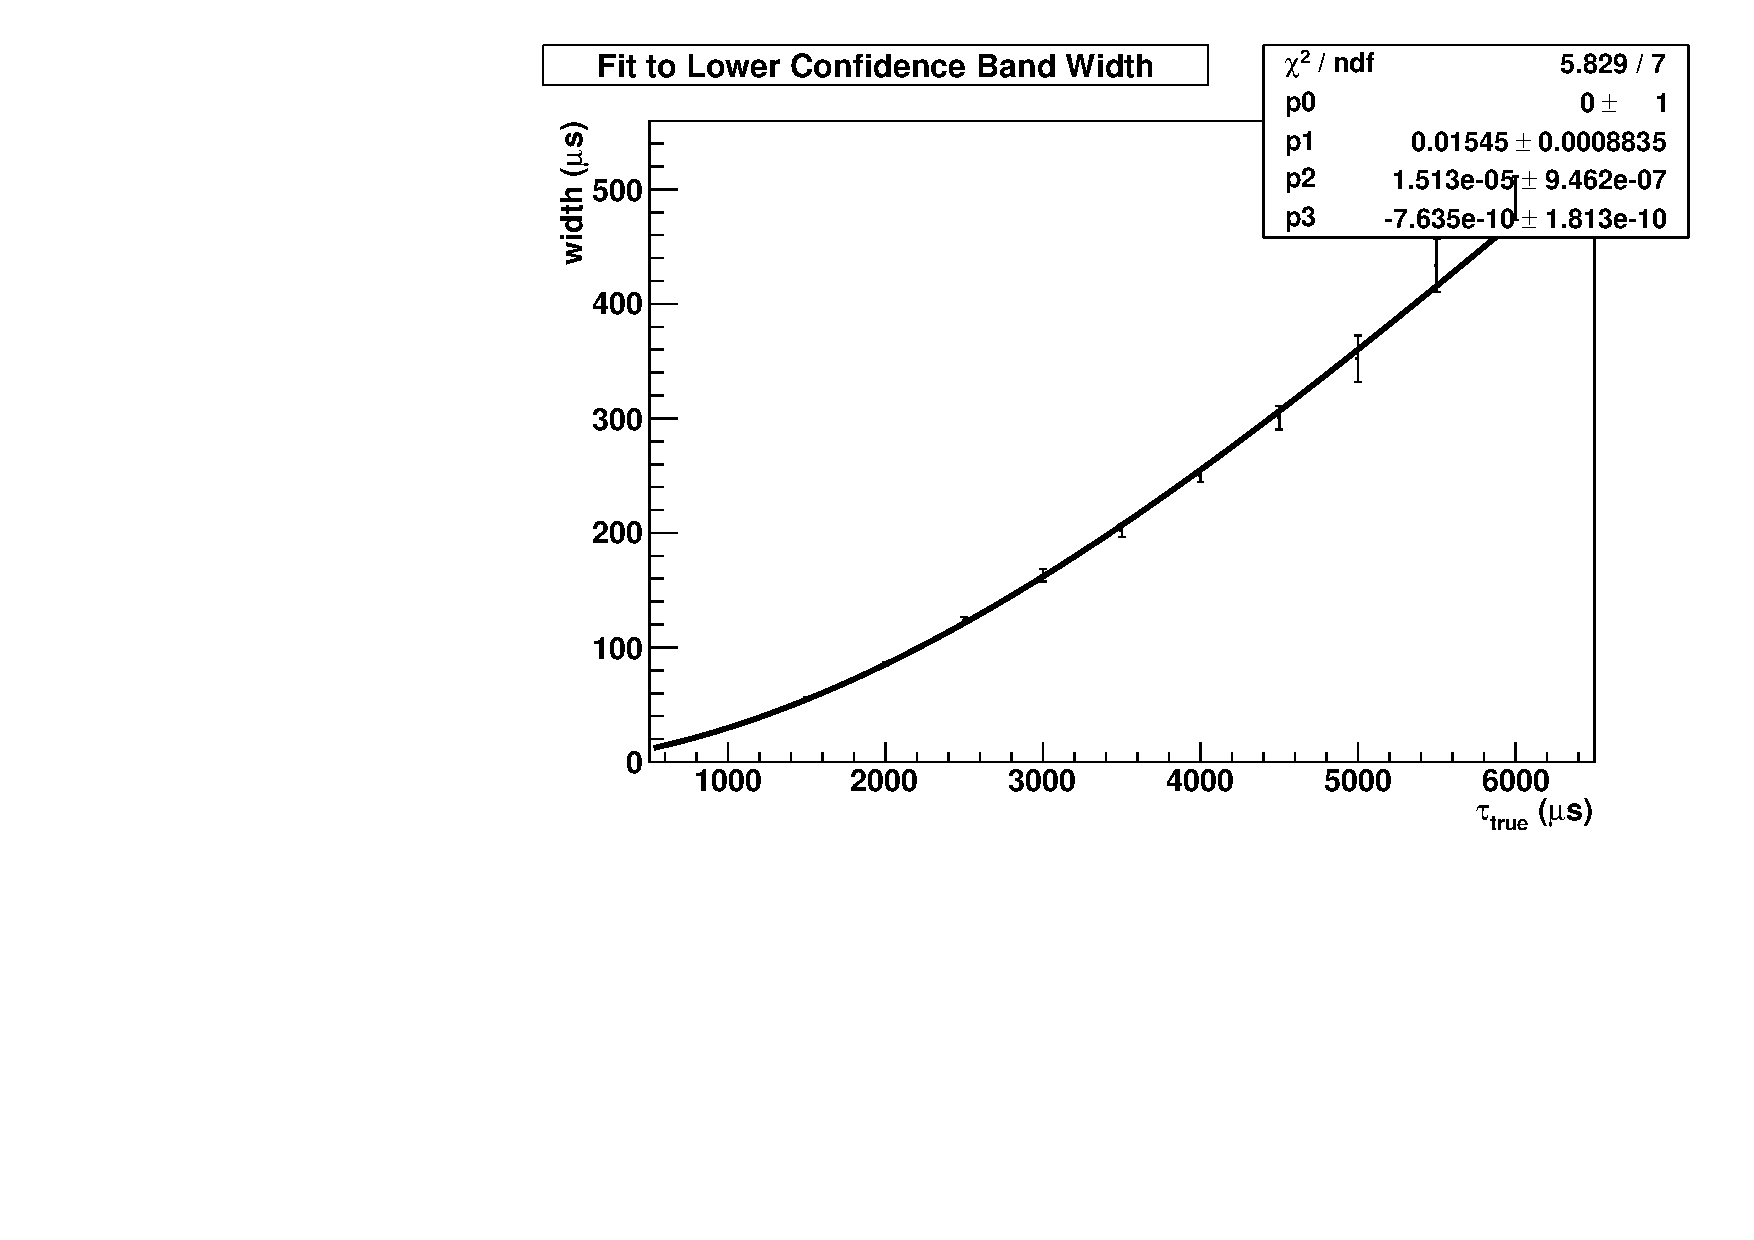
\includegraphics[width=1.0\columnwidth]{./plots/el_sim_errm_fit.pdf}
\end{subfigure}%
\begin{subfigure}[b]{0.5\linewidth}
\centering
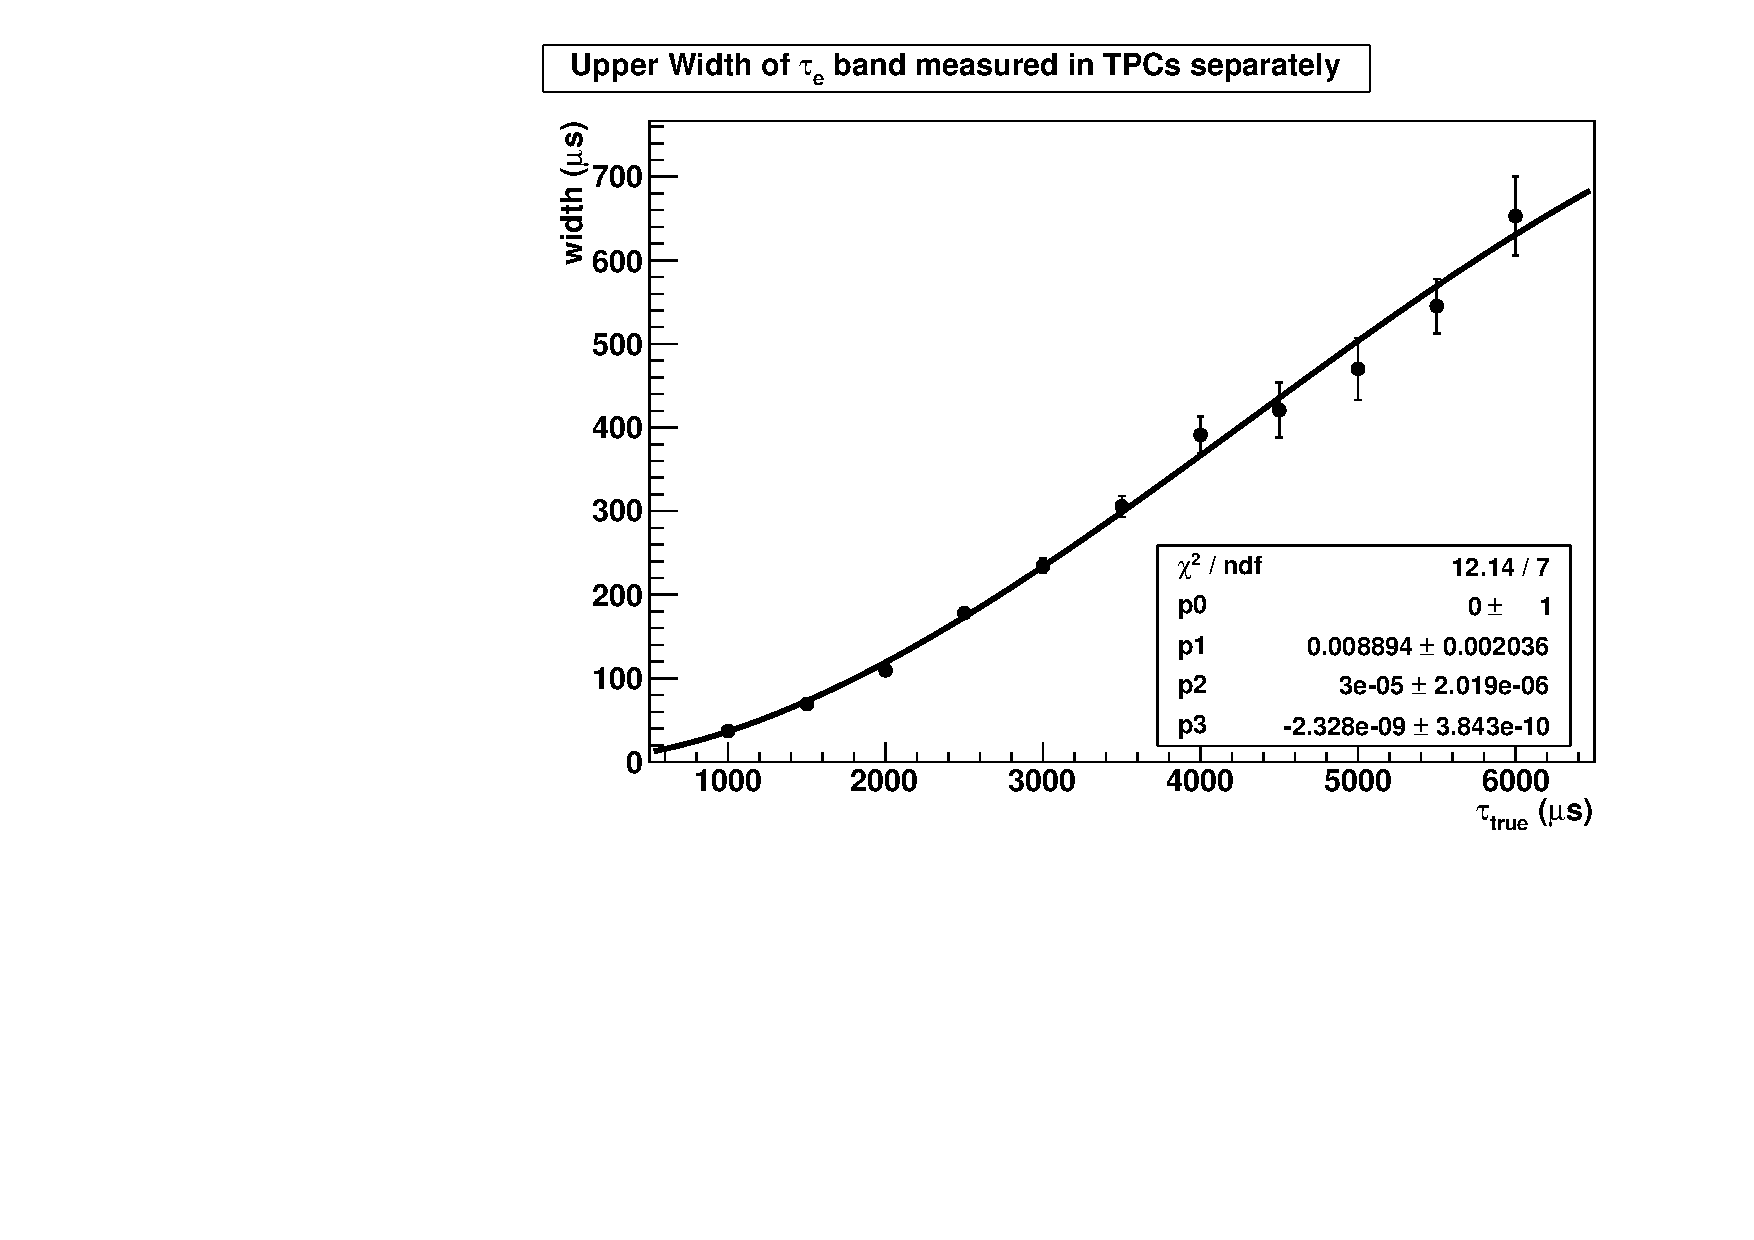
\includegraphics[width=1.0\columnwidth]{./plots/el_sim_errp_fit.pdf}
\end{subfigure}
\caption[Fits to errors on electron lifetime measurements]{The width of the uncertainty bars on single electron lifetime measurements as a function of the electron lifetime. Since the uncertainties  are asymmetric, the negative uncertainty (left) and the positive uncertainty (right) are fit separately. The fit function is a cubic polynomial.}
\label{fig:el_err_fits}
\end{figure}

As shown in \cref{fig:el_err_fits}, a polynomial function nicely fits the observed uncertainties. I tabulate the effect on electron lifetime in \cref{tab:el_res_dtau}. In practice, however, the effect will be smaller because a number of measurements go into the actual correction function applied to the data.

\begin{table}[htd]
\centering
\begin{tabular}{c|c}
	\(\tau\) (\si{\micro\second})	&	\(\Delta E / E\) (\%) 	\\ \hline
	100					&	3.88				\\
	200					&	2.15				\\
	500					&	1.11				\\
	800					&	0.86				\\
	1000					&	0.78				\\
	1500					&	0.67				\\
	2000					&	0.62				\\
	2500					&	0.59				\\
	3000					&	0.58				\\
	3500					&	0.57
\end{tabular}
\caption[Electron lifetime uncertainty effect on resolution]{The effect of the electron lifetime uncertainty on energy resolution. This is based on the parameterization shown in \cref{fig:el_err_fits}. Note that the reported resolution assumes only one measurement is used for the correction. In practice, more measurements are used, and so the effect will be smaller.}
\label{tab:el_res_dtau}
\end{table}

\subsection{Rate of Change}
The electron lifetime can vary with time. The most dramatic instances are following outages, when recirculation is resumed after a period of letting xenon stagnate. Impurities leaching out of the materials in the vessel, or from liquid xenon coming into contact with different sections of plumbing can cause the purity to degrade. When the pump is turned back on, the purity recovers over several days. Likewise, as the pump operates, it can lose pumping ability, which slows the recirculation rate.

Suppose we have two measurements, \(\tau_1 \pm \sigma_{\tau_1}\) and \(\tau_2 \pm \sigma_{\tau_2}\). The best estimate of the rate of change is simply
\[\frac{d\tau}{dt} = \frac{\tau_2 - \tau_1}{\Delta t}\]
However, the uncertainties make this slope consistent with anything within the extremes given by:
\[\frac{d\tau}{dt} = \frac{(\tau_2 \pm \sigma_{\tau_2}) - (\tau_1 \pm \sigma_{\tau_1})}{\Delta t}\]

\begin{table}[htd]
\centering
\begin{tabular}{c|c|c}
	\(\tau\) (\si{\micro\second})	&	\(d\tau/dt\) (\si{\micro\second\per\day})	&	\(\Delta E / E\) (\%) 	\\ \hline
	1000					&	10			&	0.01				\\
						&	50			&	0.03				\\
						&	100			&	0.05				\\
						&	500			&	0.27				\\ \hline
	2000					&	10			&	\(<\) 0.01			\\
						&	50			&	0.01				\\
						&	100			&	0.03				\\
						&	500			&	0.14				\\
						&	1000			&	0.29				\\ \hline
	3000					&	10			&	\(<\) 0.01			\\
						&	50			&	0.01				\\
						&	100			&	0.02				\\
						&	500			&	0.10				\\
						&	1000			&	0.20						
\end{tabular}
\caption[Electron lifetime time variance effect on resolution]{The effect of the rate of change of electron lifetime on energy resolution. This shows the additional error due to linear variation between the limits of the confidence band over 1 day, which is the typical time between calibration runs. Note that the reported resolution assumes only two measurements are used for the correction. In practice, more measurements are used, and so the effect will be smaller.}
\label{tab:el_res_dtaudt}
\end{table}

In the most extreme case, this will result in energy smearing throughout the run. \Cref{tab:el_res_dtaudt} tabulates the magnitude of this smearing.

\subsection{Overall}
The effects of electron lifetime on resolution are taken in account when selecting which runs will be used for the analysis. The guidelines are such that the resolution smearing due to the electron lifetime correction is no more than 0.5\%. Runs can be used if:
\begin{enumerate}
\item Electron lifetime is above \SI{1000}{\micro\second} (due to the effects of position uncertainty and electron lifetime uncertainty)
\item Four or more measurements all show similar electron lifetime (to reduce the effect of the electron lifetime uncertainty)
\item The electron lifetime is not be increasing at more than half its current value per day, nor decreasing at more than a quarter its current value per day (to reduce the effect of time variation)
\end{enumerate}

\section{Measurements of Electron Lifetime in EXO-200}

Calibration runs taken every 1--2 days serve to measure the electron lifetime in EXO-200. In a typical calibration run, a \thorium{228} source at the cathode creates \num{2.5d5} events in the TPC. Of these, approximately 2500 are single site events within 2\(\sigma\) of the full-absorption peak.

\subsection{Time Variation and Correction Function}

The measured electron lifetime varies in time. Usually, this variation is small and slow. To account for this, a piecewise polynomial is fit to the measured electron lifetimes. This piecewise polynomial can be discontinuous across sudden changes in electron lifetime. The polynomial degree can change when the behavior of the electron lifetime changes, such as when rapidly-increasing lifetime after resuming recirculation becomes a steady-state, slowly-varying value. \Cref{fig:el_time_variation} shows the time variation and the polynomial fit for the separate TPCs. Separate electron lifetimes are used for the different TPCs because there could be some purity gradient in the chamber, and splitting the chamber in half provides a modest approximation. Furthermore, the measured values in the different TPCs are observed to sometimes vary outside of each others' confidence bands.

\begin{figure}[htb]
\begin{subfigure}[b]{0.5\linewidth}
\centering
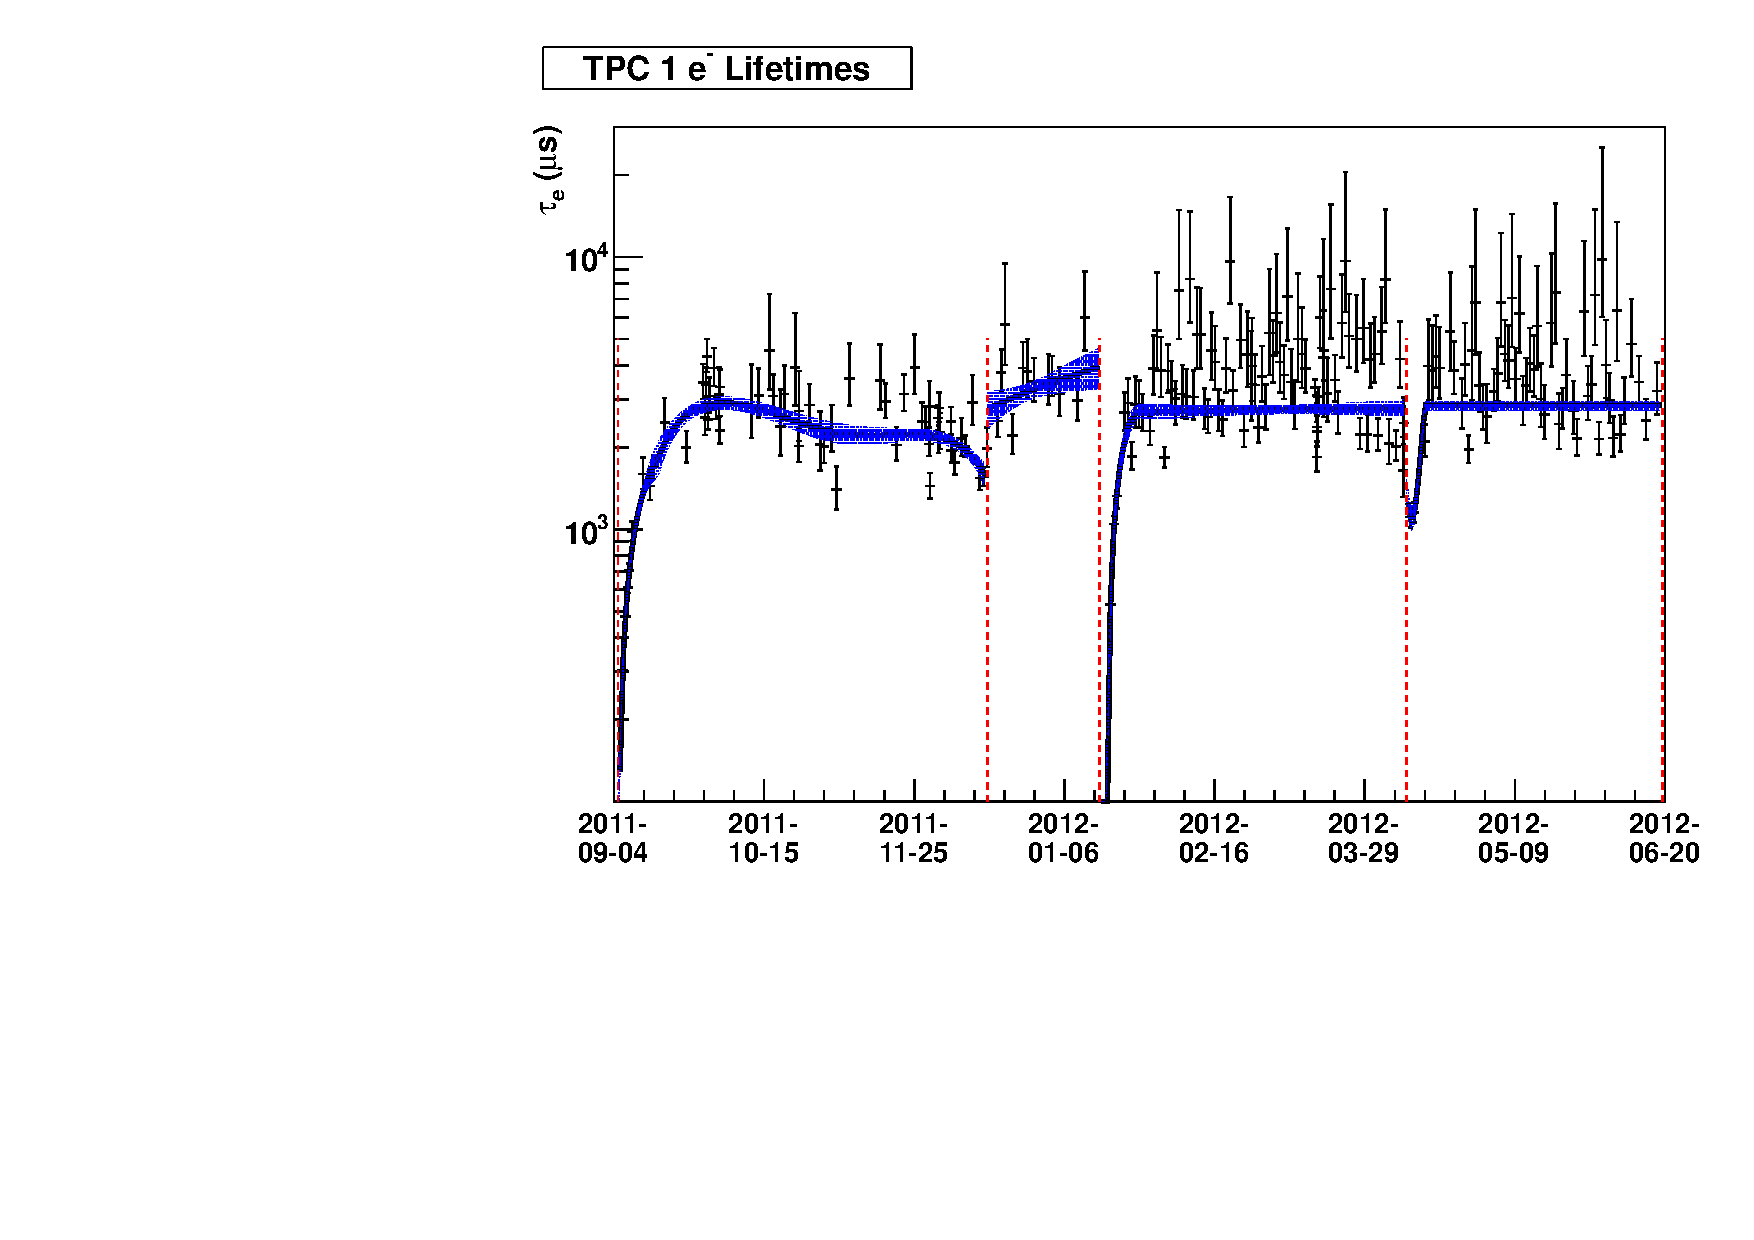
\includegraphics[width=1.0\columnwidth]{./plots/el_trend_tpc1.pdf}
\end{subfigure}%
\begin{subfigure}[b]{0.5\linewidth}
\centering
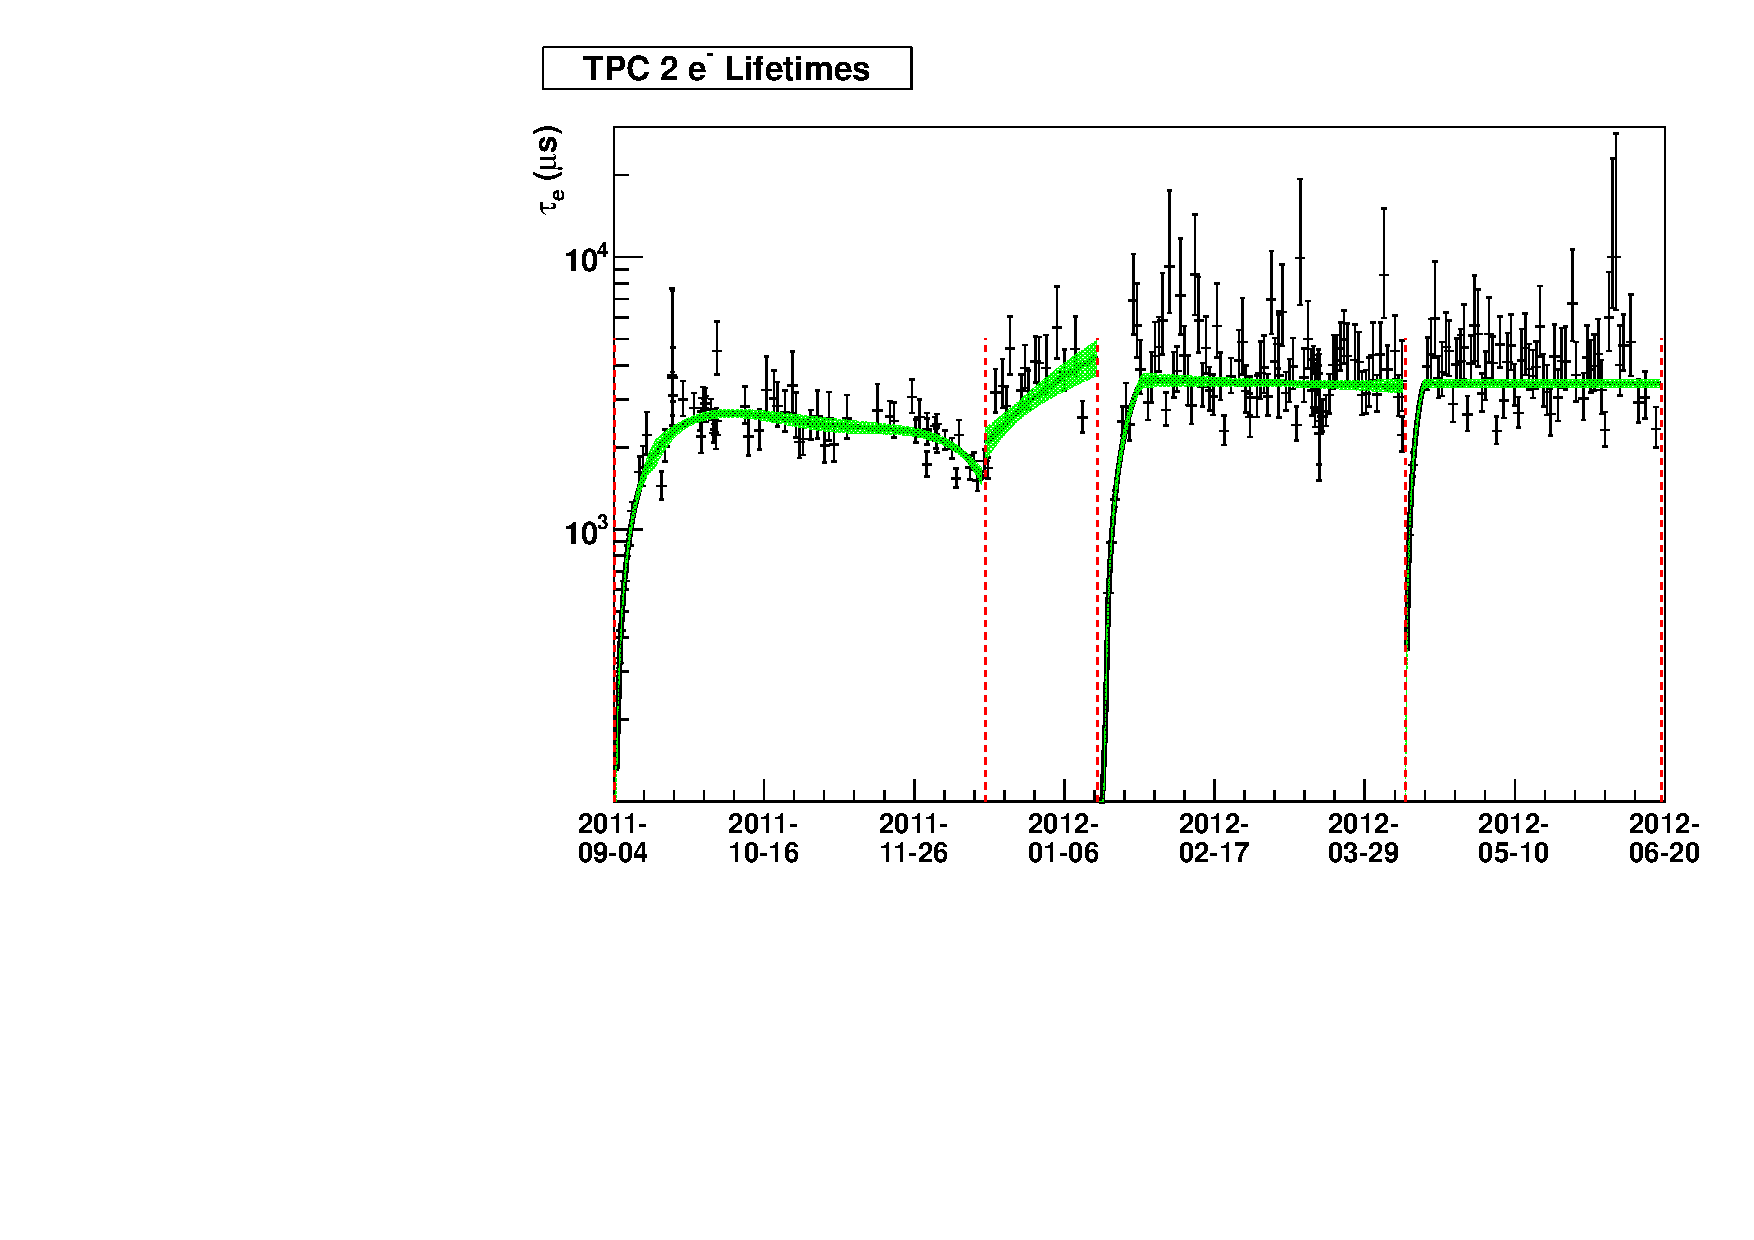
\includegraphics[width=1.0\columnwidth]{./plots/el_trend_tpc2.pdf}
\end{subfigure}
\caption[Fit to time-varying electron lifetime]{The fit of a piecewise polynomial to electron lifetime in TPC 1(left) and TPC 2 (right). The colored bands show the 68\% confidence interval on the fit. The vertical dashed lines indicate discontinuities in the electron lifetime due to pump stoppages or xenon feeds.}
\label{fig:el_time_variation}
\end{figure}

For a good event in EXO-200, the reconstruction algorithms find both a drift time and an (attenuated) ionization signal. The polynomial fit described above provides an estimate of the electron lifetime at the event time. \Cref{eq:el_exponentialtaue} provides a recipe for correcting the attenuated ionization signal to get a corrected signal, using the drift time and measured electron lifetime.

\subsection{Comparison with Recirculation Rate}
The rate at which xenon is recirculated through the purifiers effects electron lifetime. \Cref{fig:el_vs_recirculation} shows a clear trend of increasing electron lifetime with increasing recirculation rate. The highest electron lifetimes are achieved with a recirculation rate above \SI{13}{slpm}, which corresponds to completely recirculating the volume of the chamber in \SI{1.8}{days}.

\begin{figure}[htb]
\centering
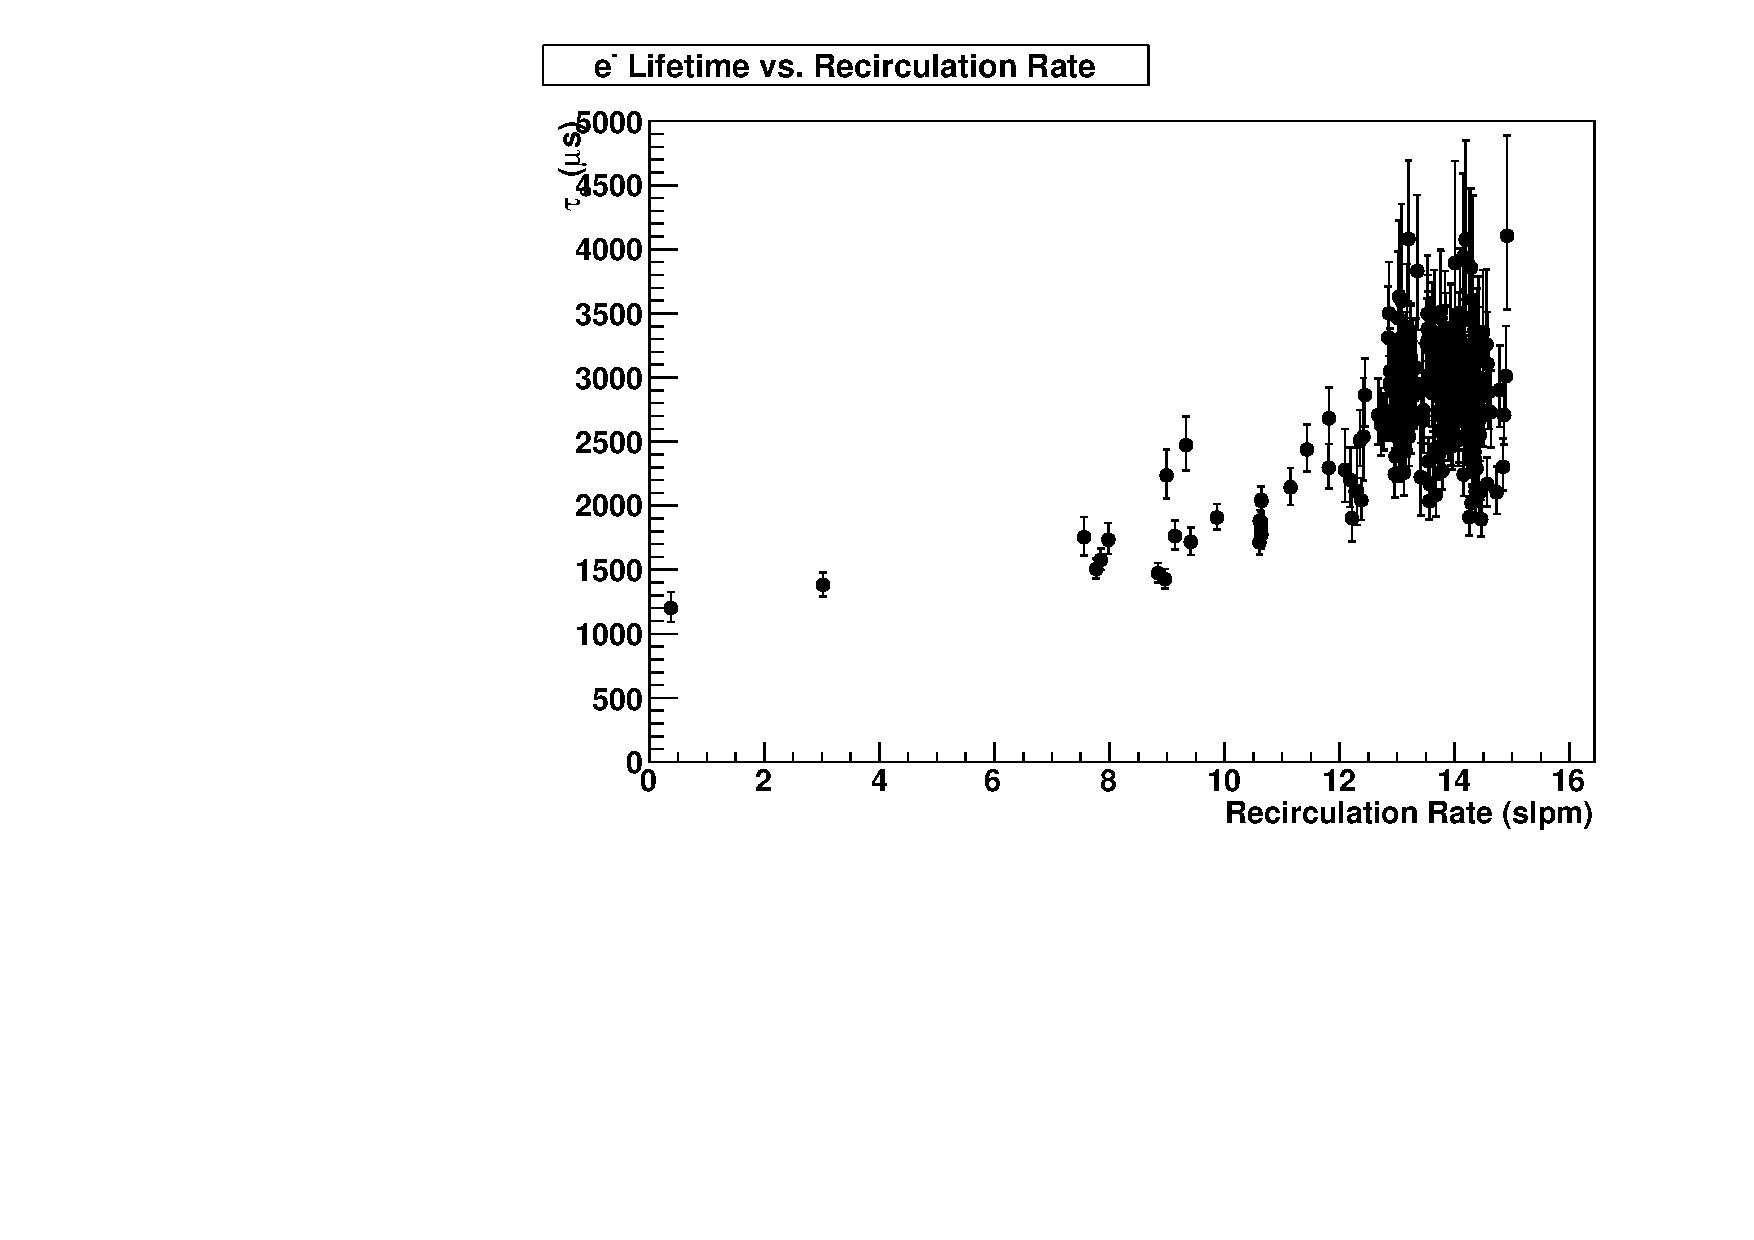
\includegraphics[width=0.6\columnwidth]{./plots/el_vs_recirculation.pdf}
\caption[Electron lifetime vs. recirculation rate]{The electron lifetime plotted as a function of recirculation rate. Time periods when recirculation was fast, but electron lifetimes were low due to a pump stoppage or feed event have been removed. A clear trend is visible, in which electron lifetime increases with recirculation rate.}
\label{fig:el_vs_recirculation}
\end{figure}

\Cref{fig:el_and_recirculation} shows the time history of the electron lifetime, plotted along with the recirculation rate. Since the electron lifetime in the chamber decreases when the pump is recirculating at a reduced rate, there is most likely a constant source of impurities in the TPC. That the electron lifetime worsens significantly after prolonged recirculation stoppages supports this. However, when the recirculation stops, the pressures throughout the system change. This causes liquid levels to change and may also cause the slow control system to feed in more gas. Newly exposed or submerged plumbing, and new gas (even though it is fed through the purifiers) could also cause this decrease in electron lifetime, and it is difficult to disentangle the effects. In any case, once recirculation is resumed, the electron lifetime recovers over the course of a few days.

\begin{figure}[htb]
\centering
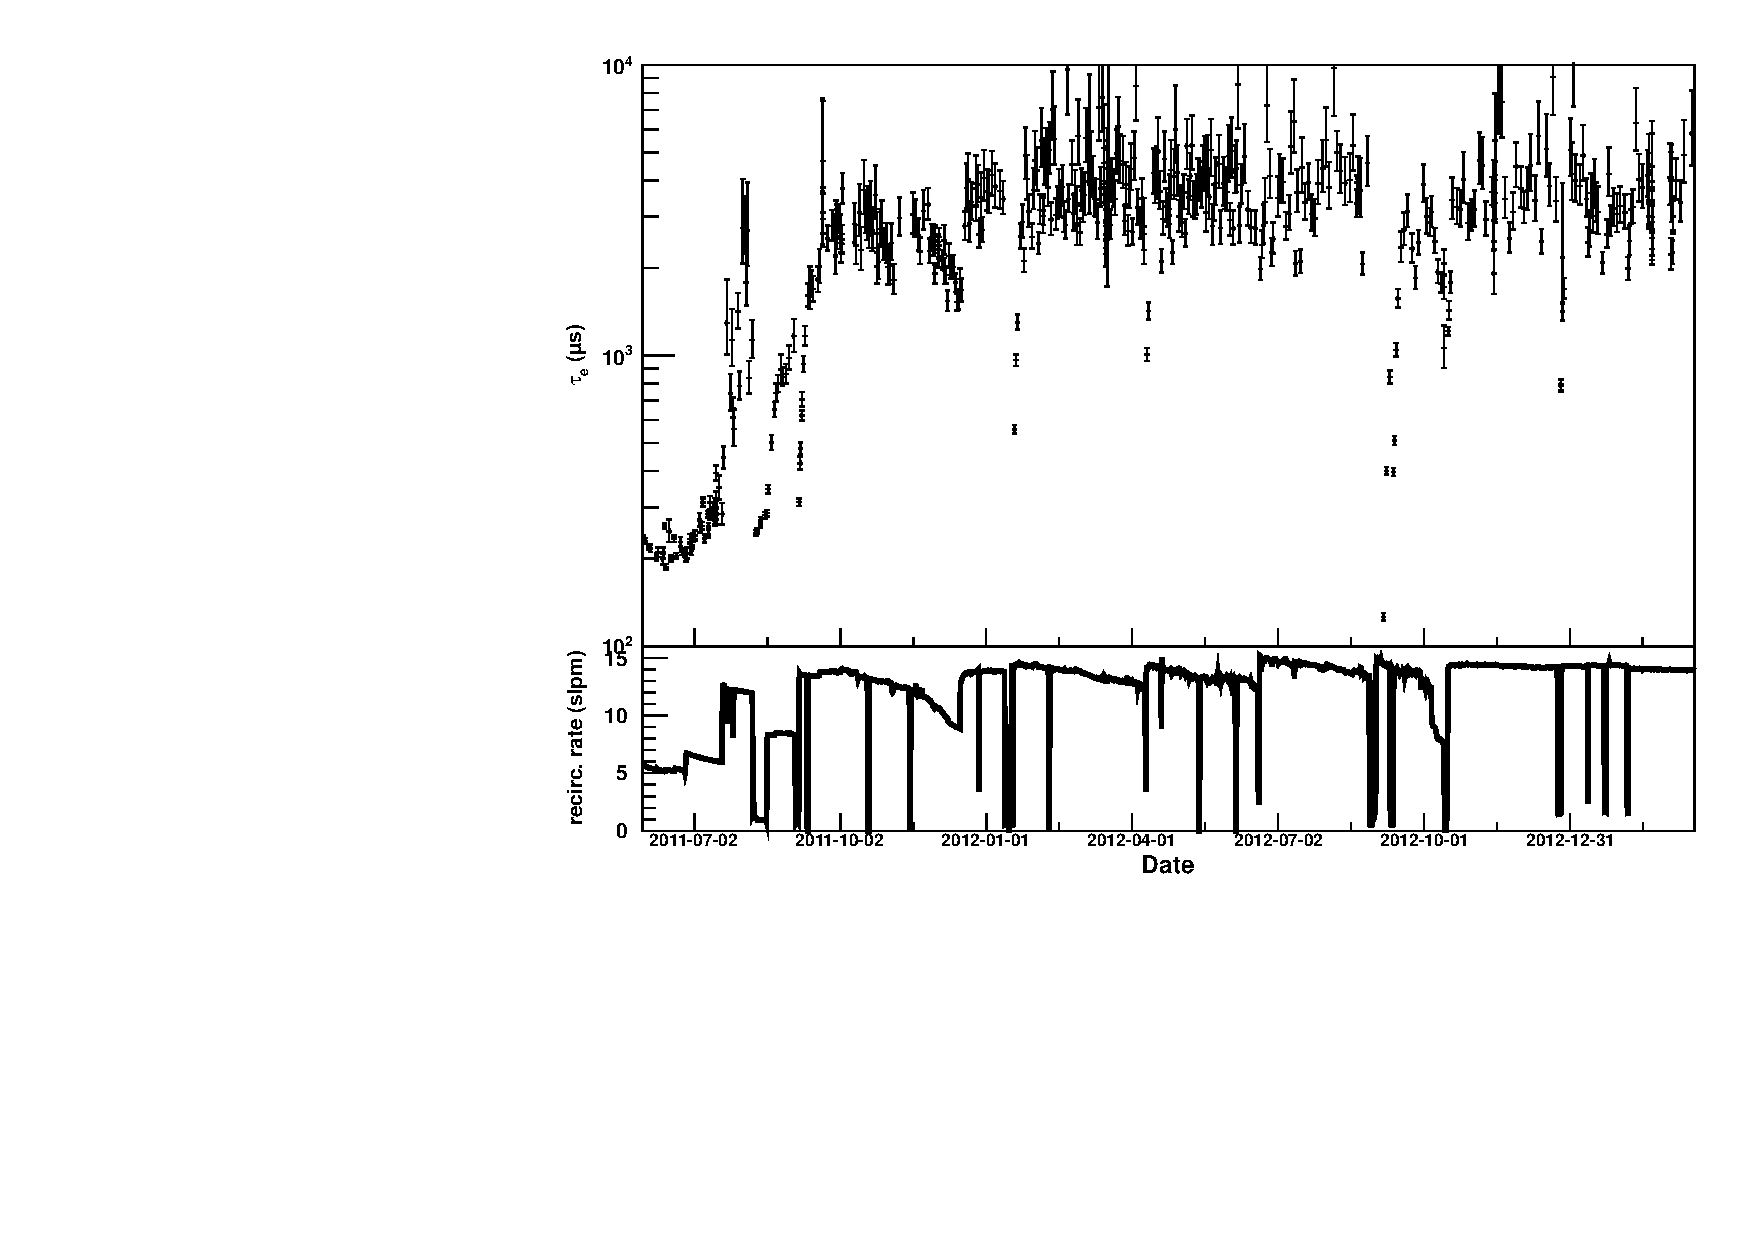
\includegraphics[width=0.6\columnwidth]{./plots/el_and_recirculation.pdf}
\caption[Electron lifetime history with recirculation rate]{A time history of the electron lifetime, with the recirculation rate plotted below. The electron lifetime drops when the pump slows or completely stops, and recovers when recirculation resumes at a fast rate.}
\label{fig:el_and_recirculation}
\end{figure}

\subsection{Comparison with Gas Purity Monitor Readings}
The gas purity monitors\cite{Dobi:2011zr} provide real-time monitoring of the recirculating xenon. GPM 1 samples the gas returning from the TPC. GPM 2 samples the gas coming out of the purifiers. GPM 3 samples the gas at the output of the recirculation pump. Because these sample room temperature gas instead of cryogenic liquid, some impurities may be in different concentrations than in the TPC due to different solubilities. Likewise, the gas purity monitors have a small electric field and short drift distance, and so they will not be able to measure long electron lifetimes. Despite this, GPM 1 may be able to provide some information about the purity of the xenon in the TPC when that purity is poor.

\begin{figure}[htb]
\centering
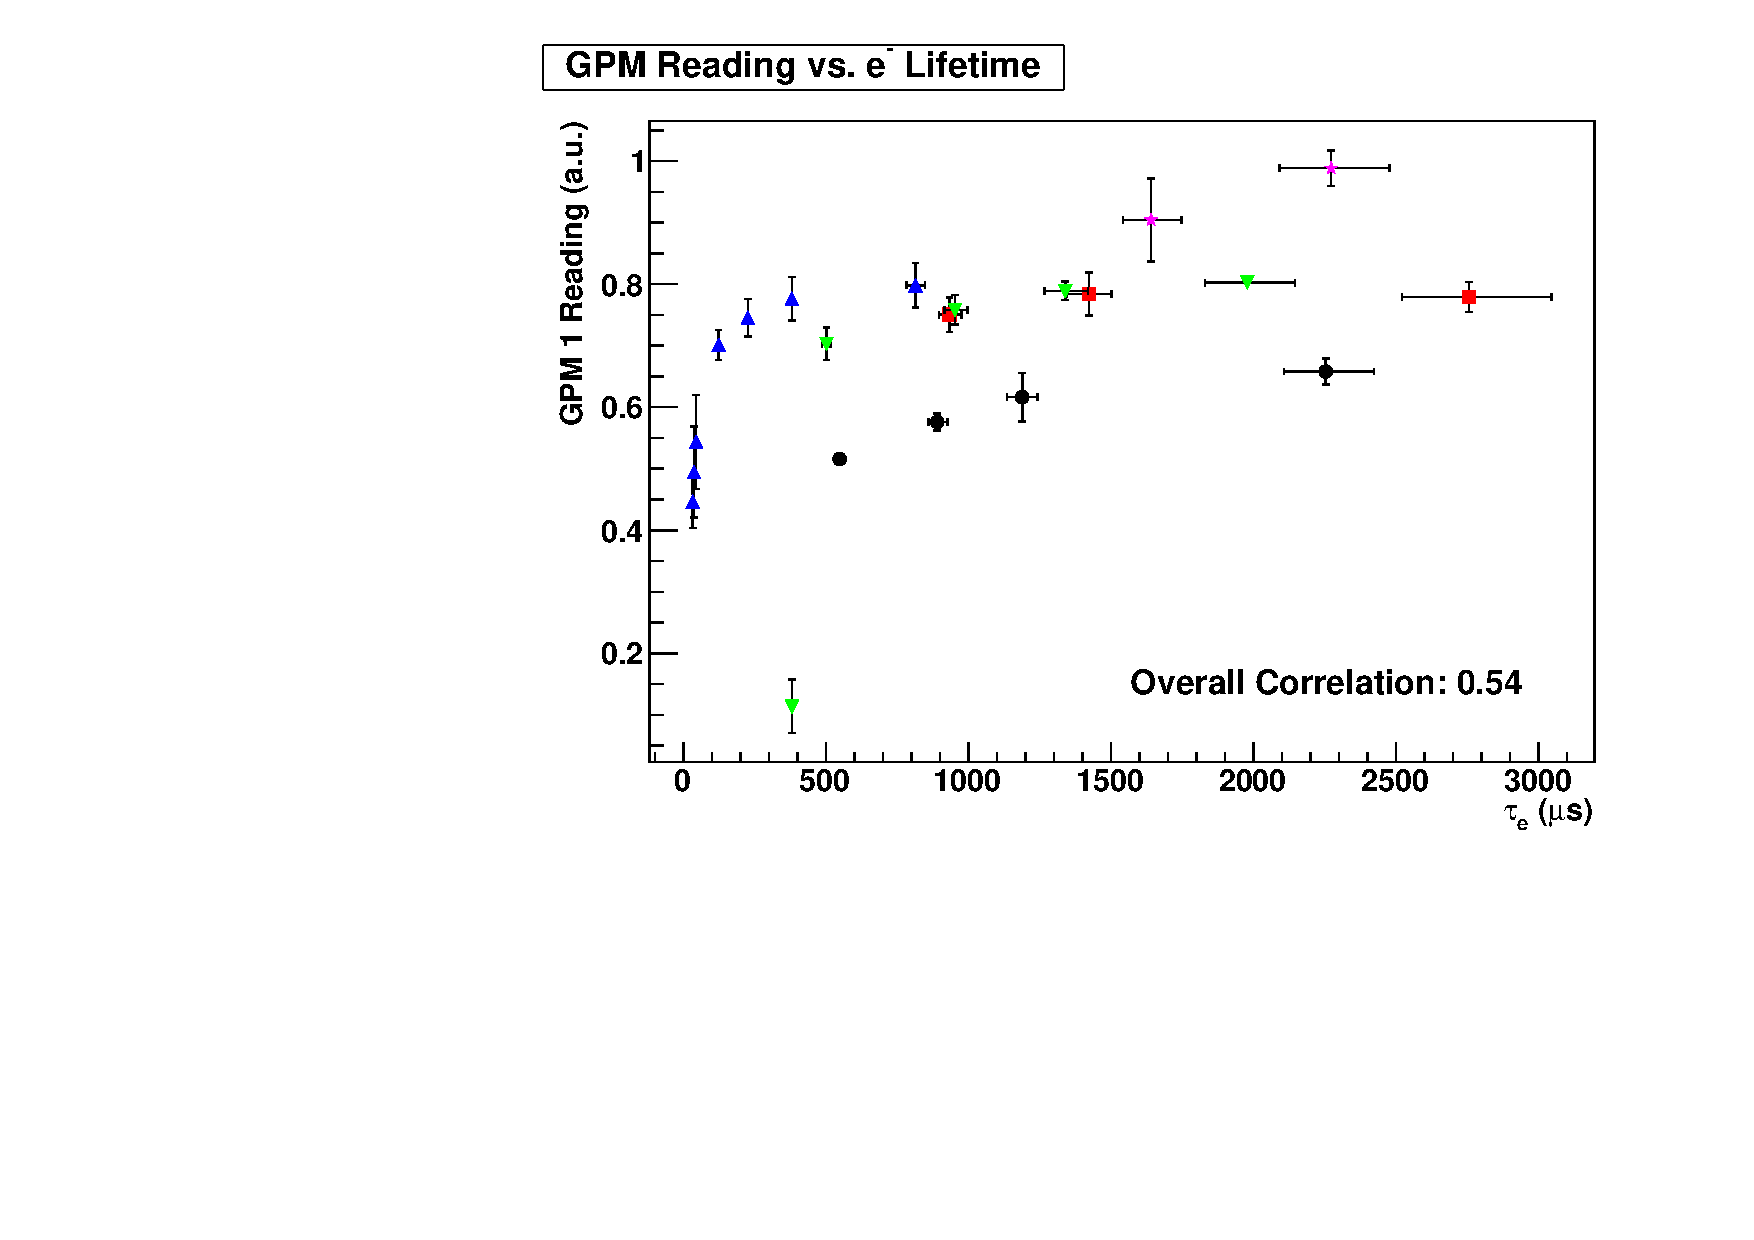
\includegraphics[width=0.6\textwidth]{./plots/el_gpm_vs_el.pdf}
\caption[GPM reading vs. electron lifetime]{The reading from the gas purity monitor sampling the gas returning from the TPC (GPM 1), during periods when the electron lifetime was recovering from a pump stoppage or feed event. Different recover incidents are denoted with different colors and markers. There is an overall correlation coefficient of 0.55 between the GPM reading and the electron lifetime. However, the correlations in individual incidents are stronger.}
\label{fig:el_gpm_vs_el}
\end{figure}

\Cref{fig:el_gpm_vs_el} shows a plot of the gas purity monitor reading for gas returning the TPC during periods when the electron lifetime was poor due to a pump stoppage or feed event. A loose correlation is visible, with a correlation coefficient of 0.55 over all points. More interesting is that the correlation is stronger during individual recovery incidents, denoted by different markers and colors. So, while the gas purity monitors do not measure the electron lifetime in the TPC on an absolute scale, they provide a good indication of large changes in the electron lifetime.

\subsection{Electron Lifetime in Low Electric Field}
The rate constant for electron attachment to impurities varies with the electric field strength, and the species of impurity determines the nature of this variation. As show in \cref{fig:el_attachment_vs_efield}\cite{Bakale:1976ly}, \ce{O_2} impurities show decreasing attachment with increasing field strength, while \ce{N_2O} show the opposite.

\begin{figure}[htb]
\centering
\begin{subfigure}[b]{0.35\linewidth}
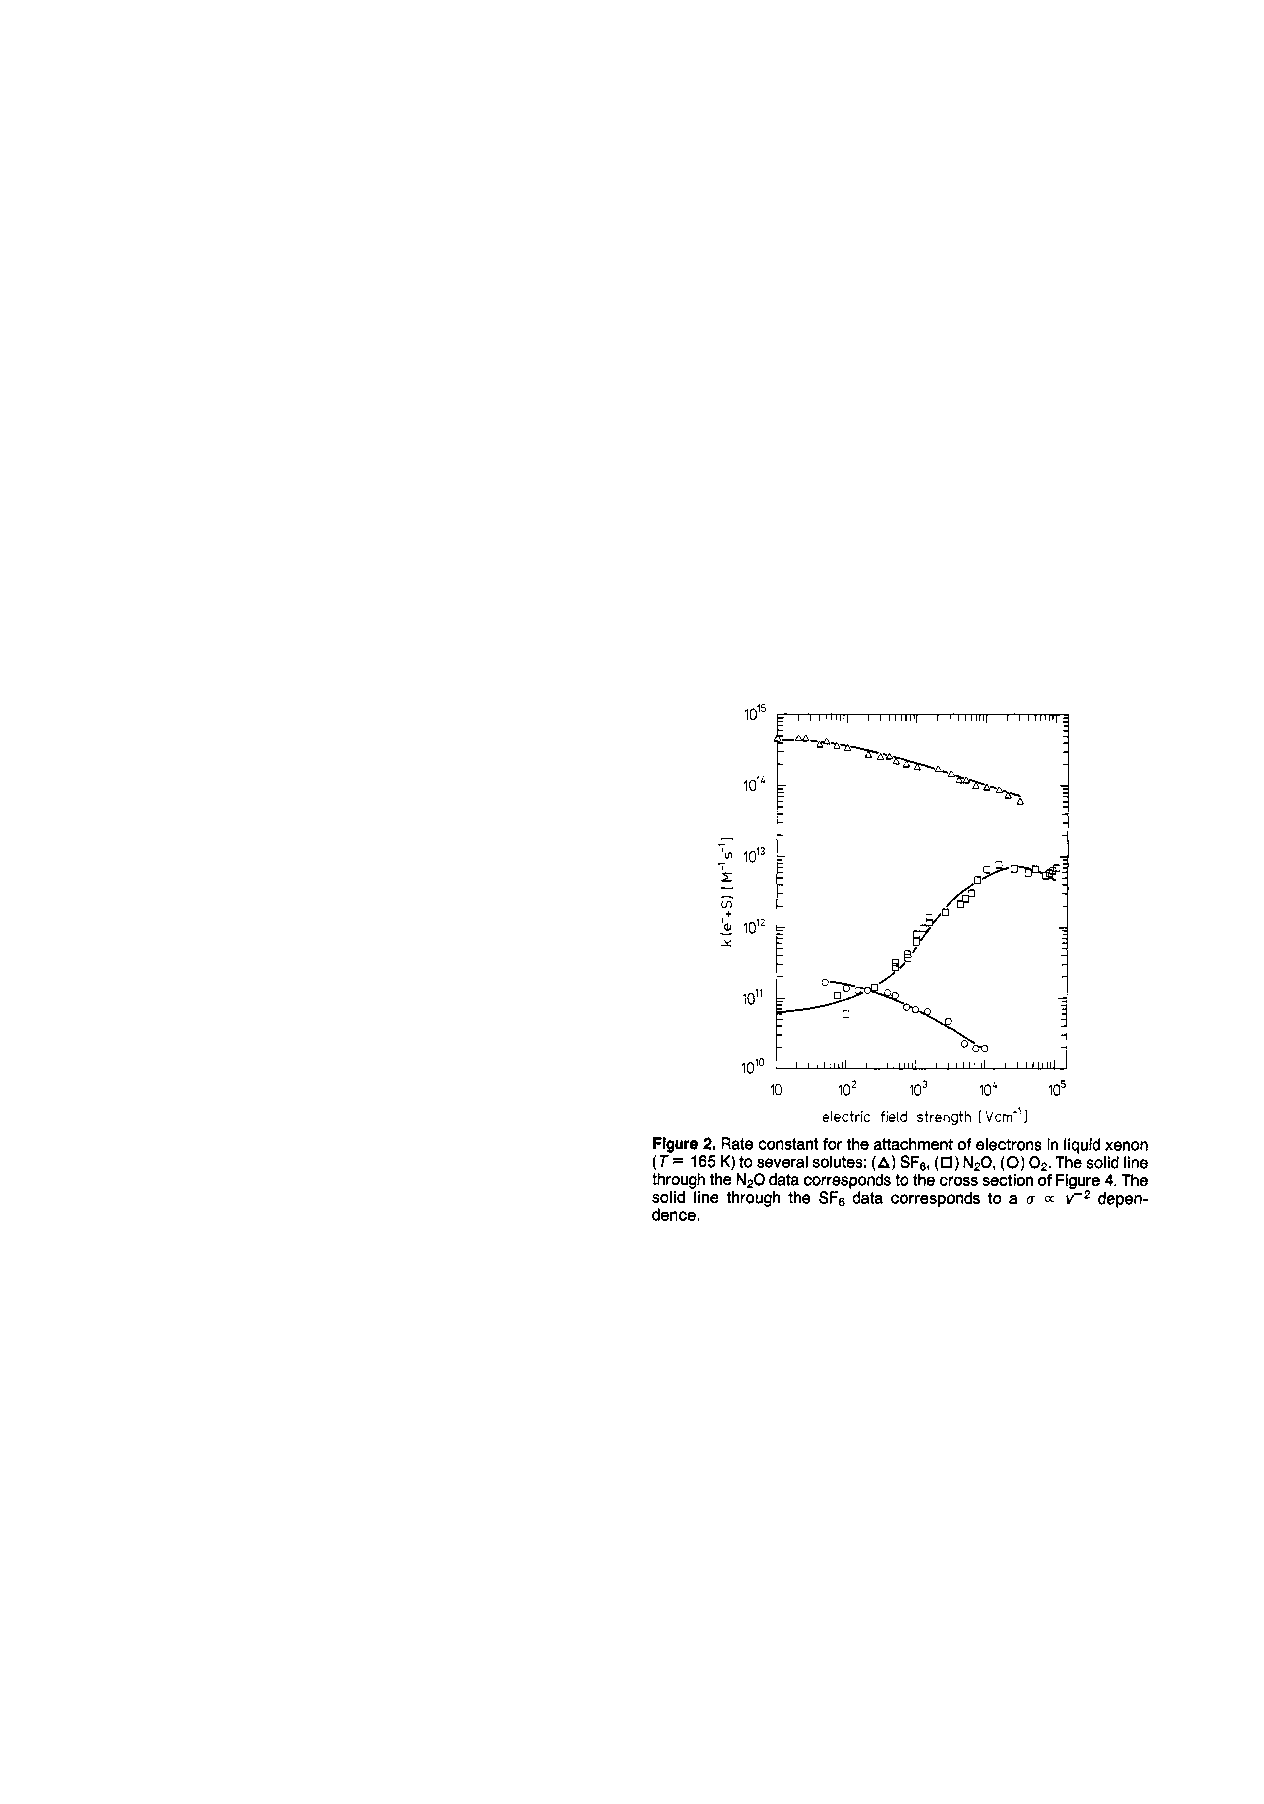
\includegraphics[width=\textwidth]{./plots/el_attachment_vs_efield.pdf}
\end{subfigure}\hspace{0.05\linewidth}%
\begin{subfigure}[b]{0.55\linewidth}
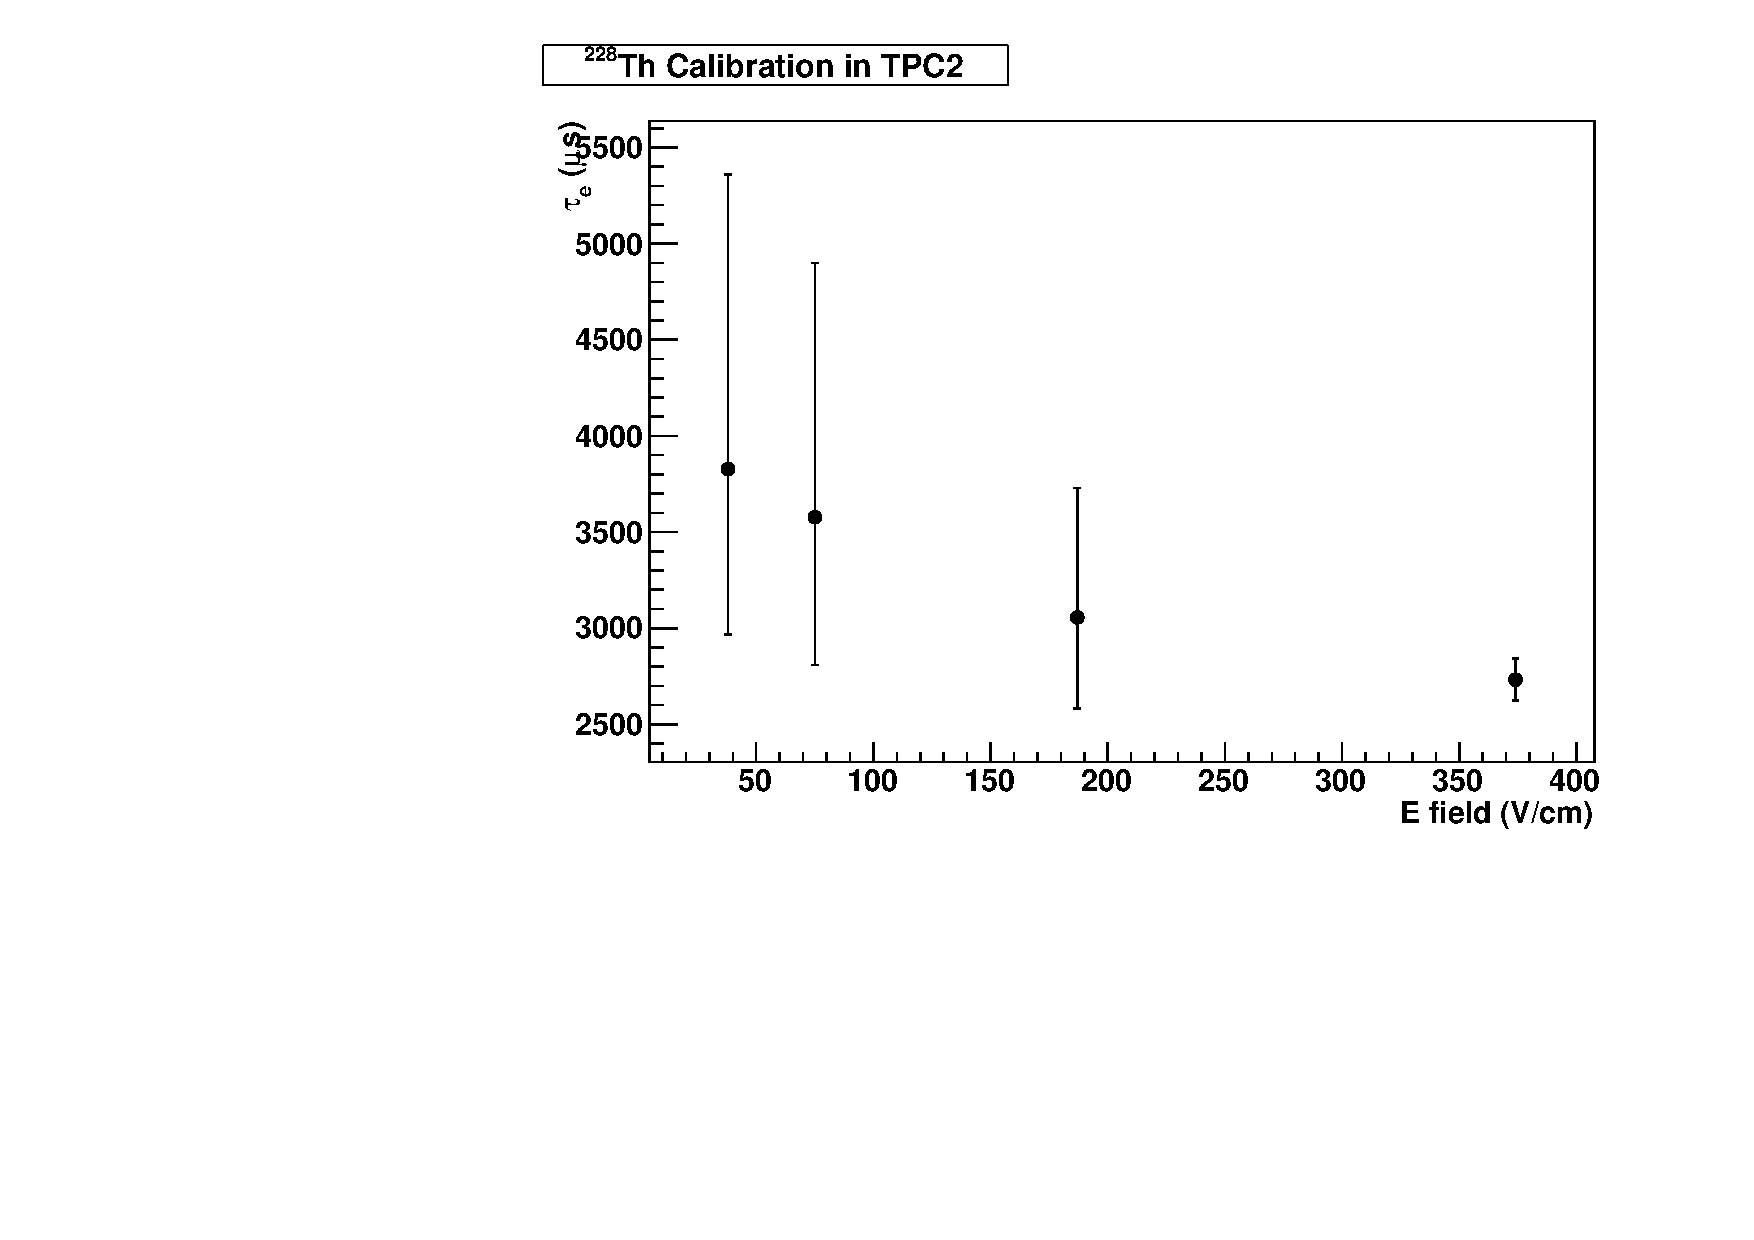
\includegraphics[width=\textwidth]{./plots/el_lifetime_vs_efield.pdf}
\end{subfigure}
\caption[Electron lifetime vs. electric field]{On the right is a plot by Bakale et al.\cite{Bakale:1976ly}, showing the electron attachment constant as a function of electric field strength. On the right is the measured electron lifetime, which is inversely proportional to the attachment constant, in EXO-200 for a number of electric field strengths. For these runs, the calibration source was located slightly on the TPC 2 side of the cathode, giving more events and allowing a better measurement in this TPC. The nominal field for normal operation is \SI{374}{\V\per\cm}. The results are not incompatible with a constant electron lifetime (\(\chi^2/\text{n.d.f.} = 3.15/3\)). However, there does seem to be a trend of decreasing electron lifetime with increasing electric field, and the magnitude of this decrease is not unreasonable, resembling \ce{N_2O}.}
\label{fig:el_attachment_vs_efield}
\label{fig:el_lifetime_vs_efield}
\end{figure}

Calibration runs of the standard length were taken with the cathode at \SIlist{-4.4;-2.2;-1.45; -1.1}{\kilo\V}, corresponding to electric field strengths of \SIlist{187;75;38;20}{\V\per\cm}. Normal operation is at \SI{-8}{\kilo\V}, corresponding to \SI{374}{\V\per\cm}. Unfortunately, there were not enough events in the full-absorption peak to measure the electron lifetime at the lowest field strength. The results are shown in \cref{fig:el_lifetime_vs_efield}. The electron lifetime seems to decrease with increasing electric field, unlike oxygen. There is not enough information to identify the exact species of impurity present. For species with similar molecular weight and electron attachment as \ce{N_2O} and \ce{O_2}, the required concentration of impurities for a \SI{3}{\ms} electron lifetime is on the order of \(10^{-11}\) (gram per gram).

%\bibliographystyle{plain}
%\bibliography{herrin-thesis}
\end{document}
